\documentclass[paper=a4, twoside=true, fontsize=11pt, chapterprefix=false]{scrbook}

%%%----------------------------------------------------------------
%%% ENCODING AND FONTS
\usepackage[utf8]{inputenc} % input encoding
\usepackage{times}          % general
\usepackage{helvet}         % sans serif
\usepackage[T1]{fontenc}    % font encoding

% %% special symbols
% \usepackage{pifont}% http://ctan.org/pkg/pifont
% \newcommand{\cmark}{\ding{51}}%
% \newcommand{\xmark}{\ding{55}}%

%%%----------------------------------------------------------------
%%% DOCUMENT INFO
%% additional variables
\makeatletter
\newcommand\reporttype[1]{\def\@reporttype{#1}}
\newcommand\timespan[1]{\def\@timespan{#1}}
\newcommand\group[1]{\def\@group{#1}}
\newcommand\supervisor[1]{\def\@supervisor{#1}}
\newcommand\chiefsupervisor[1]{\def\@chiefsupervisor{#1}}
\makeatother

%% entries
\title{Development of a Low-Cost Modal Analysis System}
\subtitle{subtitle}
\reporttype{Master Thesis}
\author{Roman Rüttimann}
\supervisor{Nino Ceresa}
\chiefsupervisor{Prof. Konrad Wegener}
\group{Institute of Machine Tools and Manufacturing}
\timespan{Spring Semester 2020}
\date{\today}

%%%----------------------------------------------------------------
%%% PATHS
\newcommand*{\texpath}{content}
\newcommand*{\imgpath}{figures}

%%%----------------------------------------------------------------
%%% INITIALIZE
%%%----------------------------------------------------------------
%%% PDF OUTPUT DETECTION
\usepackage{ifpdf}

%%%----------------------------------------------------------------
%%% COLORS
\usepackage{xcolor}       % color commands

%%%----------------------------------------------------------------
%%% MATH
\usepackage{amsmath}      % principal math package
\usepackage{amssymb}      % extended math symbols
\usepackage{amsthm}       % improved theorem definition
\usepackage{bm}           % bold greek letters
\usepackage{physics}      % simplified commands for physics notation
\usepackage{siunitx}      % consistent SI-units
  \sisetup{per-mode=symbol-or-fraction,
    range-phrase=\dots,
    range-units=single,
    binary-units=true
  }


%%%----------------------------------------------------------------
%%% LISTS
\usepackage{enumitem}
\usepackage[printonlyused]{acronym} % abbreviation list

%%%----------------------------------------------------------------
%%% FIGURES
%\usepackage{tocbasic}     % floating figures (KOMA script compatible)
%\usepackage{scrhack}      % fixes floating environments in KOMA script
%\usepackage[footnotesize, sl, SL, hang, tight]{subfigure}
\ifpdf
    \PassOptionsToPackage{pdftex}{graphicx}
\fi
\usepackage{graphicx}     % improved includegraphics
\usepackage{rotating}     % rotate graphics (load after graphicx)

%%%----------------------------------------------------------------
%%% TABLES
\usepackage{booktabs}     % better spacing
\usepackage{longtable}    % multi page tables
\usepackage{colortbl}     % allows to color cell backgrounds
\usepackage{makecell}     % for easy table headers
\usepackage{multirow}     % merge cells vertically
    \renewcommand\theadfont{\bfseries\sffamily}

% %%%----------------------------------------------------------------
% %%% CAPTIONS
\usepackage[
  font={small,sl},        % small, italic
  format=hang,            % hanging
  labelfont=bf            % bold label
  ]{caption}              % captions for tables and figures
\usepackage[%
  subrefformat=parens,
  labelformat=parens
  ]{subcaption}            % allows to do subcaptions in figures
%\usepackage{captcont}     % subfigures over multiple pages

%%%----------------------------------------------------------------
%%% PAGE STYLE
\usepackage[automark]{scrlayer-scrpage}   % enhanced header editing in KOMA-Script
\KOMAoptions{
  DIV=8,                    % type area, the larger the factor, the larger the text block
  BCOR=10mm,                % binding correction
  headinclude=true,         % insert header space
  headings=twolinechapter,  % chapter in two lines
  numbers=noenddot          % all numbers of setioning commands are set without a final point
}
%% header presets
\newpairofpagestyles{standardheadings}{%
	\ohead{\rightmark}
	\ofoot{\pagemark}
}
\newpairofpagestyles{chapterheadings}{%
	\ohead{}
	\ofoot{\pagemark}
}
\renewcommand*{\chapterpagestyle}{chapterheadings}


\usepackage{microtype}      % better text spacing

\topmargin  -12.7mm
\textheight 234.0mm
\textwidth  160.0mm
\oddsidemargin   4.57mm
\evensidemargin -5.59mm
\parskip   2.54mm
\parindent 0mm
\headsep  15mm
%\footskip 10mm

\renewcommand{\arraystretch}{1.5}
\renewcommand{\baselinestretch}{1}

%%----------------------------------------------------------------
%% BIBLIOGRAPHY
\usepackage[backend=biber,style=numeric-verb,url=false,doi=false,isbn=false]{biblatex}

%%%----------------------------------------------------------------
%%% REFERENCING

\makeatletter
\Ifpdfoutput{% (if output is pdf)
    \usepackage[%   % parse hyperref options
        pdfusetitle=false,            % disable automatic metadata
        pdftex,                       % pdftex backend
        bookmarks,                    % make bookmarks
        bookmarksopen=true,           % open bookmarks tree
        bookmarksnumbered=true,       % put section numbers in bookmarks
        pdfauthor={\@author},         % metadata, pdf author name
        pdftitle={\@title: \@subtitle}, % metadata, pdf title name
        pdfsubject={\@reporttype},    % metadata, pdf subject
        pdfproducer={Latex with hyperref}, % metadata, pdf producer
        pdfcreator={latexmk},         % metadata, pdf creator
        colorlinks=true,             % box hyperlinks
        linkcolor=black,              % textcolor of links
        citecolor=black,              % textcolor of citation links
        filecolor=black,              % textcolor of file links
        urlcolor=black,               % textcolor of url links
        anchorcolor=black,            % anchor color
        menucolor=black,              % color of menu links
        breaklinks=true,              % allow links to break over multiple lines
        pageanchor=true,              % for jumping to a page
        plainpages=false,             % page number anchors as plain arabic
        pdfpagelabels=true            % pdf page labels correspond to file
    ]{hyperref}
    \makeatother
}{% (else)
    \usepackage{hyperref}
}


%%----------------------------------------------------------------
%% TOOLKITS
% \usepackage{csquotes}     % Advanced quotation tools
\usepackage{pdfpages}     % include full pdf pages
\usepackage[mode=image]{standalone}   % include standalone tikz graphics as tex or pdf
\usepackage{tcolorbox}    % colored text boxes
  \tcbuselibrary{skins}
\usepackage{currfile}     % get path information about current file
\usepackage{tikz}
\usepackage{anyfontsize}
\usepackage{pgfplots}
\pgfplotsset{compat=1.17}

\begin{comment}
%%%----------------------------------------------------------------
%%% BIBLIOGRAPHY URL LINKS
% format that applies a hypertext reference
\DeclareFieldFormat{linked}{%
  \ifboolexpr{ test {\ifhyperref} and not test {\ifentrytype{online}} }
    {\iffieldundef{doi}
       {\iffieldundef{url}
          {\iffieldundef{isbn}
             {\iffieldundef{issn}
                {#1}
                {\href{https://portal.issn.org/resource/ISSN/\thefield{issn}}{#1}}}
             {\href{https://books.google.com/books?vid=ISBN\thefield{isbn}}{#1}}}
          {\href{\thefield{url}}{#1}}}
       {\href{http://dx.doi.org/\thefield{doi}}{#1}}}
    {#1}}

% Define new command that returns the first word of a given field
\makeatletter
\def\thefieldfirstword#1{%
  \expandafter\expandafter
  \expandafter\firstword
  \expandafter\expandafter
  \expandafter{\csname abx@field@#1\endcsname}}
\def\firstword#1{\firstword@i#1 \@nil}
\def\firstword@i#1 #2\@nil{#1}
\makeatother

% Redefine url format to print only first URL, omit URL prefix
\DeclareFieldFormat{url}{\url{\firstword{#1}}}

\renewbibmacro*{title}{% Based on generic definition from biblatex.def
  \ifboolexpr{ test {\iffieldundef{title}} and test {\iffieldundef{subtitle}} }
    {}
    {\printtext[title]{\printtext[linked]{%
       \printfield[titlecase]{title}%
       \setunit{\subtitlepunct}%
       \printfield[titlecase]{subtitle}}}%
     \newunit}%
  \printfield{titleaddon}}

\renewbibmacro*{periodical}{% Based on generic definition from biblatex.def
  \iffieldundef{title}
    {}
    {\printtext[title]{\printtext[linked]{%
       \printfield[titlecase]{title}%
       \setunit{\subtitlepunct}%
       \printfield[titlecase]{subtitle}}}}}

% Don't link titles in citations
\AtEveryCite{\DeclareFieldAlias{linked}{default}}
\end{comment}
\pdfcompresslevel=9
\pdfoutput=1
\DeclareGraphicsExtensions{.pdf,.png}

%%%----------------------------------------------------------------
%%% HEADERS
%\definecolor{laccentcolor}{HTML}{d3d3d3}

\renewcommand*{\chapterheadstartvskip}{\vspace{7cm}}
\addtokomafont{disposition}{\sffamily}
\addtokomafont{chapter}{\huge}

\newif\ifappendix

\def\chaplengths{{11mm,6mm,7mm,2.5mm,7mm,5mm,6mm,7mm,6.5mm}}
\def\applengths{{4mm,8.5mm,6mm}}
\renewcommand*{\chapterformat}{%
	\begin{tikzpicture}[remember picture, overlay]
		\pgfmathsetmacro{\mylength}{\ifappendix\applengths[\arabic{chapter}-1]\else\chaplengths[\arabic{chapter}-1]\fi}
    	\node(n)[anchor=north east, inner sep=0, outer sep=1cm,
        	font=\fontsize{3.4cm}{3.4cm}\selectfont, align=right%,text=laccentcolor
			  ] at (\linewidth+1cm, 6cm) {\hfill \rule{0pt}{\ht\strutbox}\thechapter};
    	\pgfresetboundingbox
    	\useasboundingbox(n.south west)rectangle([xshift=-\mylength]n.north east);% bounding box with a fixed height
	\end{tikzpicture}%
}

%%%----------------------------------------------------------------
%%% TITLE PAGE
\makeatletter
\renewcommand\maketitle{%
    \pagestyle{empty}
    \begin{center}
    %\includegraphics*[width=0.38\textwidth]{figures/title/ETH_logo}
    \includegraphics*[scale=1]{figures/title/eth_logo_hardcopy}
    \hfill
    % Choose your logo here!
    %\includegraphics*[width=0.37\textwidth]{figures/title/iwf_eth_logo}
    %\includegraphics*[width=0.21\textwidth]{figures/title/loco_icvr}
    %\includegraphics*[width=0.21\textwidth]{figures/title/logo_inspire_ics}
    %\includegraphics*[width=0.24\textwidth]{figures/title/logo_inspire_icvr}
    %\includegraphics*[width=0.24\textwidth]{figures/title/logo_inspire_irpd}
    \includegraphics*[scale=1]{figures/title/iwf_logo_hardcopy}
    \vspace{6cm}
    \newline
	\Huge
	\textbf{\textsf{\@title}}\\[0.7cm]
	%\Large\@subtitle\\[2.0cm]
	%\includegraphics*[width=0.4\textwidth]{figures/title/mytitlefigure}
	\vspace{1cm}
	\sffamily\Large
    \@author\\[0.7cm]
	\large\@reporttype\\[0.7cm]
	\@supervisor\\
	\@chiefsupervisor\\[0.7cm]
	%\begin{tabular}[t]{rl}
	%    supervisor: & \@supervisor\\
	%    chief supervisor: & \@chiefsupervisor
	%\end{tabular}\\[0.7cm]
	\@group
	\end{center}
}
\makeatother

% %% CHAPTER (with numbering)
% \titleformat{\chapter}[block]
%     {\normalfont\Large\bfseries}    % format applied to label+text
%     {}                              % label
%     {1pc}                           % horizontal separation between label and title body
%     {%
%         \noindent\parbox[][4cm][t]{\textwidth - 4\fboxsep}{%
%             \begin{flushright}
%                 \begin{tcolorbox}[
%                     standard jigsaw,
%                     flushright upper,
%                     boxrule=0pt,
%                     frame hidden,
%                     opacityback=0,
%                     width=2.8cm]
%                     \resizebox{1.8cm}{!}{\color{black}\thechapter}%
%                 \end{tcolorbox}
%             \end{flushright}
%         }\\\Huge
%     }                               % before the title body
%     []                              % after the title body

% %% CHAPTER (without numbering)
% \titleformat{name=\chapter,numberless}
%     {\normalfont\Large\bfseries}   % format applied to label+text
%     {\hspace{-1em}}                % label, fix for horizontal spacing
%     {1pc}                          % horizontal separation between label and title body
%     {%
%         \noindent\parbox[][4cm][t]{\textwidth - 4\fboxsep}{%
%         }\\\Huge
%     }                              % before the title body
%     []                             % after the title body

% \addtokomafont{paragraph}{\sffamily}

% \def\mychpstyleintl{%
% {\noindent\setlength{\tabcolsep}{0pt}\setlength{\arrayrulewidth}{2pt}%
% \begin{tabular}{c}
% \\[100pt]
% \begin{tabular}{lr}
% \begin{tabular}{p{0.6\linewidth}}
% \\
% \end{tabular}
% &
% \begin{tabular}{p{0.4\linewidth}}
% \rightline{{%
% \sffamily%
% \fontseries{bx}%
% \fontshape{n}%
% \fontsize{100}{120}%choose baselineskip to be 1.2 times font size
% \selectfont
% \thechapter}}
% \end{tabular}
% \end{tabular}\\[300pt]
% \end{tabular}
% }}
                       % loads all usepackages and changes layout
% commands
\newcommand{\Adjoint}{\mbox{\rm Adj}}
\newcommand{\Area}{\mbox{\rm Area}}
\newcommand{\ACos}{{\mbox{\rm Cos}^{-1}}}
\newcommand{\ASin}{{\mbox{\rm Sin}^{-1}}}
\newcommand{\ATan}{{\mbox{\rm atan2}}}
\newcommand{\Code}[1]{{\tt #1}}
\newcommand{\Complex}{\mbox{\bf C}}
\newcommand{\Cross}{{\mbox{\rm Cross}}}
\newcommand{\Mydddot}[1]{\mbox{\shortstack{$.$\hspace*{-1pt}$.$\hspace*{-1pt}$.$\\$#1$}}}
\newcommand{\Degree}{\mbox{\rm degree}}
\newcommand{\Diag}{\mbox{\rm Diag}}
\newcommand{\Dim}{\mbox{\rm dim}}
\newcommand{\Dist}{\mbox{\rm Distance}}
\newcommand{\IntTwo}{\int\!\!\int}
\newcommand{\IntThree}{\int\!\!\int\! \!\int}
\newcommand{\Kernel}{\mbox{\rm kernel}}
\newcommand{\Kross}{\mbox{\rm Kross}}
\newcommand{\Grad}{\nabla}
\newcommand{\Perp}{\mbox{\rm Perp}}
\newcommand{\Point}[1]{{\cal #1}}
\newcommand{\Rank}{\mbox{\rm rank}}
\newcommand{\Range}{\mbox{\rm range}}
\newcommand{\Real}{{\mbox{\rm I}\hspace*{-2pt}\mbox{\rm R}}}
\newcommand{\RealSbt}{{\mbox{\rm\scriptsize I}\hspace*{-2pt}\mbox{\rm\scriptsize R}}}
\newcommand{\Res}{\mbox{\rm resultant}}
\newcommand{\Sbt}[1]{{\mbox{\rm\scriptsize #1}}}
\newcommand{\MySign}{\mbox{\rm Sign}}
\newcommand{\SignSBT}{\mbox{\rm\scriptsize Sign}}
\newcommand{\Skew}{\mbox{\rm Skew}}
\newcommand{\Span}{\mbox{\rm Span}}
\newcommand{\SqrDist}{\mbox{\rm Distance$^2$}}
\newcommand{\Trace}{\mbox{\rm Trace}}
\newcommand{\TRN}{{\mbox{\rm\scriptsize T}}}
\newcommand{\Vector}[1]{\mbox{\bf #1}}
\newcommand{\VectorM}[1]{\mbox{\boldmath $#1$}}
\newcommand{\Volume}{\mbox{\rm Volume}}

\newcommand{\IVec}{\mbox{\boldmath $\imath$}}
\newcommand{\JVec}{\mbox{\boldmath $\jmath$}}
\newcommand{\KVec}{\mbox{\boldmath $k$}}
\newcommand{\LVec}{\mbox{\boldmath $\ell$}}
\newcommand{\RMat}{{\cal R}}
\newcommand{\QMat}{{\cal Q}}
\newcommand{\QCMat}{\overline{\cal Q}}

\newcommand{\Lerp}{\mbox{\rm lerp}}
\newcommand{\Slerp}{\mbox{\rm slerp}}
\newcommand{\Quad}{\mbox{\rm quad}}
\newcommand{\Squad}{\mbox{\rm squad}}

\newcommand{\subsubsubsection}[1]{{\sc #1}}

\newcommand{\ODer}[2]{\frac{d #1}{d #2}}
\newcommand{\ODerT}[2]{\frac{d^2 #1}{d {#2}^2}}
\newcommand{\ODerM}[3]{\frac{d #1}{d #2 \, d #3}}
\newcommand{\PDer}[2]{\frac{\partial #1}{\partial #2}}
\newcommand{\PDerT}[2]{\frac{\partial^2 #1}{\partial {#2}^2}}
\newcommand{\PDerM}[3]{\frac{\partial^2 #1}{\partial #2 \, \partial #3}}

% mass density symbol
\newcommand{\Den}{\delta}

% environments
\newenvironment{BArray}[1]{\left\{ \begin{array}{#1}}{\end{array} \right\}}
\newenvironment{Combin}{\left( \begin{array}{c}}{\end{array} \right)}
\newenvironment{Matrix}[1]{\left[ \begin{array}{#1}}{\end{array} \right]}

% "Figure" environment
\newtheorem{localFigure}{Figure}[chapter]
\newenvironment{Figure}[1]{
  \begin{center}
  \begin{minipage}{6in}
  \par\noindent\hspace*{0pt}\hrulefill
  
  \begin{localFigure} \label{#1}
}{
  \end{localFigure}
  \par\noindent\hspace*{0pt}\hrulefill
  \end{minipage}
  \end{center}
}

% "Table" environment
\newtheorem{localTable}{Table}[chapter]
\newenvironment{Table}[1]{
  \begin{center}
  \begin{minipage}{6in}
  
  \begin{localTable} \label{#1}
}{
  \end{localTable}
  \end{minipage}
  \end{center}
}

% "CDROM" environment for source code on disk
%\newenvironment{CDROM}[1]{
%  \label{#1} 
%    \includegraphics{cdrom.png} \hspace*{0.1in}{\tt PointShop3D}. \rm
%}{
%  $\bowtie$
%}

% TO DO search symbol
\newcommand{\TODO}{\mbox{\large\bf TO DO}}
\newcommand{\REFR}{\mbox{\large\bf REFR}}

%  Terminates current page and paragraph, makes sure next page starts on
%  an odd-number, and generates a completely blank page, without page markers,
%  if necessary.
\newcommand{\clearemptydoublepage}{\newpage{\pagestyle{empty}\cleardoublepage}}

%%% Shoemake's commands
\DeclareMathOperator{\prp}{\text{\scshape perp}}
\DeclareMathOperator{\rot}{rot}
\DeclareMathOperator{\N}{N}
\providecommand{\vmag}[1]{\lVert#1\rVert}
\providecommand{\mutate}[1]{\overleftarrow{#1}}
\providecommand{\T}[1]{{#1}^{\mathrm T}}
\newcommand{\cross}{\times}
\newcommand{\by}{\times}
\newcommand{\vect}[1]{\mathbf{#1}}
\newcommand{\mat}[1]{\mathbf{#1}} % or not
%\newcommand{\quat}[1]{\mathbf{#1}}
\newcommand{\quat}[1]{\ensuremath{\mathbf{\dot{#1}}}}
\newcommand{\vV}{\vect{v}}
\newcommand{\vU}{\vect{u}}
\newcommand{\vE}{\vect{e}}
\newcommand{\vUh}{\hat{\vect{u}}}
\newcommand{\mQ}{\mat{Q}}
\newcommand{\mR}{\mat{R}}
\newcommand{\mM}{\mat{M}}
\newcommand{\mA}{\mat{A}}
\newcommand{\mB}{\mat{B}}
\newcommand{\mI}{\mat{I}}
\newcommand{\mJ}{\mat{J}}
\newcommand{\mX}{\mat{X}}
\newcommand{\mY}{\mat{Y}}
\newcommand{\mZ}{\mat{Z}}
\newcommand{\qo}{\quat{1}}
\newcommand{\qi}{\quat{i}}
\newcommand{\qj}{\quat{j}}
\newcommand{\qk}{\quat{k}}
\newcommand{\xh}{{x}}
\newcommand{\yh}{{y}}
\newcommand{\zh}{{z}}
\newcommand{\ch}{c}
\newcommand{\sh}{s}
\newcommand{\gt}{\theta}


%%
%%
%%

\definecolor{ZissouSTD5qual0}{RGB}{0,153,230}
\definecolor{ZissouSTD5qual1}{RGB}{18,37,90}
\definecolor{ZissouSTD5qual2}{RGB}{242,56,20}
\definecolor{ZissouSTD5qual3}{RGB}{223,183,139}
\definecolor{ZissouSTD5qual4}{RGB}{182,195,197}
\definecolor{ZissouL5qual0}{RGB}{59,189,255}
\definecolor{ZissouL5qual1}{RGB}{38,78,190}
\definecolor{ZissouL5qual2}{RGB}{245,115,90}
\definecolor{ZissouL5qual3}{RGB}{232,204,173}
\definecolor{ZissouL5qual4}{RGB}{203,212,214}
\definecolor{ZissouUL5qual0}{RGB}{185,231,255}
\definecolor{ZissouUL5qual1}{RGB}{171,188,238}
\definecolor{ZissouUL5qual2}{RGB}{251,205,196}
\definecolor{ZissouUL5qual3}{RGB}{247,237,226}
\definecolor{ZissouUL5qual4}{RGB}{236,240,240}
\definecolor{ZissouSTD5div0}{RGB}{84,142,169}
\definecolor{ZissouSTD5div1}{RGB}{128,174,190}
\definecolor{ZissouSTD5div2}{RGB}{224,198,54}
\definecolor{ZissouSTD5div3}{RGB}{210,168,33}
\definecolor{ZissouSTD5div4}{RGB}{212,58,15}
\definecolor{ZissouL5div0}{RGB}{134,176,195}
\definecolor{ZissouL5div1}{RGB}{166,198,209}
\definecolor{ZissouL5div2}{RGB}{233,215,114}
\definecolor{ZissouL5div3}{RGB}{229,197,93}
\definecolor{ZissouL5div4}{RGB}{241,107,69}
\definecolor{ZissouUL5div0}{RGB}{212,226,233}
\definecolor{ZissouUL5div1}{RGB}{223,234,238}
\definecolor{ZissouUL5div2}{RGB}{247,240,204}
\definecolor{ZissouUL5div3}{RGB}{245,234,197}
\definecolor{ZissouUL5div4}{RGB}{250,202,188}
\definecolor{WesMixSTD8qual0}{RGB}{82,119,130}
\definecolor{WesMixSTD8qual1}{RGB}{193,117,55}
\definecolor{WesMixSTD8qual2}{RGB}{218,170,44}
\definecolor{WesMixSTD8qual3}{RGB}{66,59,100}
\definecolor{WesMixSTD8qual4}{RGB}{43,93,71}
\definecolor{WesMixSTD8qual5}{RGB}{80,147,177}
\definecolor{WesMixSTD8qual6}{RGB}{147,31,40}
\definecolor{WesMixSTD8qual7}{RGB}{116,123,116}
\definecolor{WesMixL8qual0}{RGB}{127,163,174}
\definecolor{WesMixL8qual1}{RGB}{214,158,112}
\definecolor{WesMixL8qual2}{RGB}{229,195,107}
\definecolor{WesMixL8qual3}{RGB}{111,100,163}
\definecolor{WesMixL8qual4}{RGB}{78,169,129}
\definecolor{WesMixL8qual5}{RGB}{132,179,200}
\definecolor{WesMixL8qual6}{RGB}{214,63,74}
\definecolor{WesMixL8qual7}{RGB}{157,162,157}
\definecolor{WesMixUL8qual0}{RGB}{209,222,226}
\definecolor{WesMixUL8qual1}{RGB}{240,220,204}
\definecolor{WesMixUL8qual2}{RGB}{245,233,202}
\definecolor{WesMixUL8qual3}{RGB}{203,199,222}
\definecolor{WesMixUL8qual4}{RGB}{191,225,210}
\definecolor{WesMixUL8qual5}{RGB}{211,227,235}
\definecolor{WesMixUL8qual6}{RGB}{240,186,190}
\definecolor{WesMixUL8qual7}{RGB}{220,222,220}
\definecolor{CustomSTD8qual0}{RGB}{228,26,28}
\definecolor{CustomSTD8qual1}{RGB}{55,126,184}
\definecolor{CustomSTD8qual2}{RGB}{77,175,74}
\definecolor{CustomSTD8qual3}{RGB}{152,78,163}
\definecolor{CustomSTD8qual4}{RGB}{255,127,0}
\definecolor{CustomSTD8qual5}{RGB}{255,255,51}
\definecolor{CustomSTD8qual6}{RGB}{166,86,40}
\definecolor{CustomSTD8qual7}{RGB}{247,129,191}
\definecolor{CustomL8qual0}{RGB}{236,94,95}
\definecolor{CustomL8qual1}{RGB}{108,165,211}
\definecolor{CustomL8qual2}{RGB}{128,200,126}
\definecolor{CustomL8qual3}{RGB}{185,127,194}
\definecolor{CustomL8qual4}{RGB}{255,165,76}
\definecolor{CustomL8qual5}{RGB}{255,255,112}
\definecolor{CustomL8qual6}{RGB}{213,131,83}
\definecolor{CustomL8qual7}{RGB}{249,166,210}
\definecolor{CustomUL8qual0}{RGB}{248,197,198}
\definecolor{CustomUL8qual1}{RGB}{202,222,239}
\definecolor{CustomUL8qual2}{RGB}{209,235,209}
\definecolor{CustomUL8qual3}{RGB}{230,209,233}
\definecolor{CustomUL8qual4}{RGB}{255,223,191}
\definecolor{CustomUL8qual5}{RGB}{255,255,204}
\definecolor{CustomUL8qual6}{RGB}{240,210,193}
\definecolor{CustomUL8qual7}{RGB}{253,223,239}
\definecolor{ETHpptSTD12qual0}{RGB}{0,0,0}
\definecolor{ETHpptSTD12qual1}{RGB}{255,255,255}
\definecolor{ETHpptSTD12qual2}{RGB}{114,121,28}
\definecolor{ETHpptSTD12qual3}{RGB}{18,105,176}
\definecolor{ETHpptSTD12qual4}{RGB}{145,5,106}
\definecolor{ETHpptSTD12qual5}{RGB}{111,111,100}
\definecolor{ETHpptSTD12qual6}{RGB}{168,50,45}
\definecolor{ETHpptSTD12qual7}{RGB}{0,122,150}
\definecolor{ETHpptSTD12qual8}{RGB}{149,96,19}
\definecolor{ETHpptSTD12qual9}{RGB}{255,255,255}
\definecolor{ETHpptSTD12qual10}{RGB}{18,105,176}
\definecolor{ETHpptSTD12qual11}{RGB}{140,182,60}
\definecolor{ETHpptL12qual0}{RGB}{76,76,76}
\definecolor{ETHpptL12qual1}{RGB}{255,255,255}
\definecolor{ETHpptL12qual2}{RGB}{195,207,49}
\definecolor{ETHpptL12qual3}{RGB}{54,153,234}
\definecolor{ETHpptL12qual4}{RGB}{246,11,181}
\definecolor{ETHpptL12qual5}{RGB}{155,155,144}
\definecolor{ETHpptL12qual6}{RGB}{211,95,91}
\definecolor{ETHpptL12qual7}{RGB}{3,207,255}
\definecolor{ETHpptL12qual8}{RGB}{227,152,42}
\definecolor{ETHpptL12qual9}{RGB}{255,255,255}
\definecolor{ETHpptL12qual10}{RGB}{54,153,234}
\definecolor{ETHpptL12qual11}{RGB}{175,208,113}
\definecolor{ETHpptUL12qual0}{RGB}{191,191,191}
\definecolor{ETHpptUL12qual1}{RGB}{255,255,255}
\definecolor{ETHpptUL12qual2}{RGB}{233,238,181}
\definecolor{ETHpptUL12qual3}{RGB}{183,218,247}
\definecolor{ETHpptUL12qual4}{RGB}{251,167,228}
\definecolor{ETHpptUL12qual5}{RGB}{219,219,215}
\definecolor{ETHpptUL12qual6}{RGB}{239,198,196}
\definecolor{ETHpptUL12qual7}{RGB}{164,238,255}
\definecolor{ETHpptUL12qual8}{RGB}{245,218,179}
\definecolor{ETHpptUL12qual9}{RGB}{255,255,255}
\definecolor{ETHpptUL12qual10}{RGB}{183,218,247}
\definecolor{ETHpptUL12qual11}{RGB}{226,238,204}

\pgfplotsset{/pgfplots/colormap={ZissouSTD5qual}{%
	rgb255=(0,153,230)
	rgb255=(18,37,90)
	rgb255=(242,56,20)
	rgb255=(223,183,139)
	rgb255=(182,195,197)
}}
\pgfplotsset{/pgfplots/colormap={ZissouL5qual}{%
	rgb255=(59,189,255)
	rgb255=(38,78,190)
	rgb255=(245,115,90)
	rgb255=(232,204,173)
	rgb255=(203,212,214)
}}
\pgfplotsset{/pgfplots/colormap={ZissouUL5qual}{%
	rgb255=(185,231,255)
	rgb255=(171,188,238)
	rgb255=(251,205,196)
	rgb255=(247,237,226)
	rgb255=(236,240,240)
}}
\pgfplotsset{/pgfplots/colormap={ZissouSTD5div}{%
	rgb255=(84,142,169)
	rgb255=(128,174,190)
	rgb255=(224,198,54)
	rgb255=(210,168,33)
	rgb255=(212,58,15)
}}
\pgfplotsset{/pgfplots/colormap={ZissouL5div}{%
	rgb255=(134,176,195)
	rgb255=(166,198,209)
	rgb255=(233,215,114)
	rgb255=(229,197,93)
	rgb255=(241,107,69)
}}
\pgfplotsset{/pgfplots/colormap={ZissouUL5div}{%
	rgb255=(212,226,233)
	rgb255=(223,234,238)
	rgb255=(247,240,204)
	rgb255=(245,234,197)
	rgb255=(250,202,188)
}}
\pgfplotsset{/pgfplots/colormap={WesMixSTD8qual}{%
	rgb255=(82,119,130)
	rgb255=(193,117,55)
	rgb255=(218,170,44)
	rgb255=(66,59,100)
	rgb255=(43,93,71)
	rgb255=(80,147,177)
	rgb255=(147,31,40)
	rgb255=(116,123,116)
}}
\pgfplotsset{/pgfplots/colormap={WesMixL8qual}{%
	rgb255=(127,163,174)
	rgb255=(214,158,112)
	rgb255=(229,195,107)
	rgb255=(111,100,163)
	rgb255=(78,169,129)
	rgb255=(132,179,200)
	rgb255=(214,63,74)
	rgb255=(157,162,157)
}}
\pgfplotsset{/pgfplots/colormap={WesMixUL8qual}{%
	rgb255=(209,222,226)
	rgb255=(240,220,204)
	rgb255=(245,233,202)
	rgb255=(203,199,222)
	rgb255=(191,225,210)
	rgb255=(211,227,235)
	rgb255=(240,186,190)
	rgb255=(220,222,220)
}}
\pgfplotsset{/pgfplots/colormap={CustomSTD8qual}{%
	rgb255=(228,26,28)
	rgb255=(55,126,184)
	rgb255=(77,175,74)
	rgb255=(152,78,163)
	rgb255=(255,127,0)
	rgb255=(255,255,51)
	rgb255=(166,86,40)
	rgb255=(247,129,191)
}}
\pgfplotsset{/pgfplots/colormap={CustomL8qual}{%
	rgb255=(236,94,95)
	rgb255=(108,165,211)
	rgb255=(128,200,126)
	rgb255=(185,127,194)
	rgb255=(255,165,76)
	rgb255=(255,255,112)
	rgb255=(213,131,83)
	rgb255=(249,166,210)
}}
\pgfplotsset{/pgfplots/colormap={CustomUL8qual}{%
	rgb255=(248,197,198)
	rgb255=(202,222,239)
	rgb255=(209,235,209)
	rgb255=(230,209,233)
	rgb255=(255,223,191)
	rgb255=(255,255,204)
	rgb255=(240,210,193)
	rgb255=(253,223,239)
}}
\pgfplotsset{/pgfplots/colormap={ETHpptSTD12qual}{%
	rgb255=(0,0,0)
	rgb255=(255,255,255)
	rgb255=(114,121,28)
	rgb255=(18,105,176)
	rgb255=(145,5,106)
	rgb255=(111,111,100)
	rgb255=(168,50,45)
	rgb255=(0,122,150)
	rgb255=(149,96,19)
	rgb255=(255,255,255)
	rgb255=(18,105,176)
	rgb255=(140,182,60)
}}
\pgfplotsset{/pgfplots/colormap={ETHpptL12qual}{%
	rgb255=(76,76,76)
	rgb255=(255,255,255)
	rgb255=(195,207,49)
	rgb255=(54,153,234)
	rgb255=(246,11,181)
	rgb255=(155,155,144)
	rgb255=(211,95,91)
	rgb255=(3,207,255)
	rgb255=(227,152,42)
	rgb255=(255,255,255)
	rgb255=(54,153,234)
	rgb255=(175,208,113)
}}
\pgfplotsset{/pgfplots/colormap={ETHpptUL12qual}{%
	rgb255=(191,191,191)
	rgb255=(255,255,255)
	rgb255=(233,238,181)
	rgb255=(183,218,247)
	rgb255=(251,167,228)
	rgb255=(219,219,215)
	rgb255=(239,198,196)
	rgb255=(164,238,255)
	rgb255=(245,218,179)
	rgb255=(255,255,255)
	rgb255=(183,218,247)
	rgb255=(226,238,204)
}}

 % imports predefined colors
\addbibresource{references.bib}     % loads bibliography
\newlength{\distTextWidth}          % effective textwidth
\newlength{\distColSep}             % separation gap when using multiple columns
\setlength{\distTextWidth}{\dimexpr\textwidth-\columnsep\relax}
\setlength{\distColSep}{6pt}

%%%----------------------------------------------------------------
%%% DEBUGGING
%\usepackage{showkeys}       % DEBUGGING show labels above references
%\usepackage{comment}        % DEBUGGING comment out code with comment environment
%\usepackage{lipsum}         % DEBUGGING blind text
\usepackage{todonotes}

%%%----------------------------------------------------------------
%%% MACROS
\newcommand{\mykeyword}[0]{my long text}
%reference macros -> change this if you write you thesis in an other language!!!
\newcommand{\chpref}[1]{Chapter \ref{#1}}
\newcommand{\secref}[1]{Section \ref{#1}}
%\newcommand{\equref}[1]{Equation \ref{#1}} %better use builtin \eqref{} !!!
\newcommand{\figref}[1]{Figure \ref{#1}}
\newcommand{\tabref}[1]{Table \ref{#1}}
\newcommand{\apxref}[1]{Appendix \ref{#1}}

\begin{document}

%%%----------------------------------------------------------------
%%% TITLE PAGE
\maketitle
\cleardoublepage

%%%----------------------------------------------------------------
%%% PREFACE
\frontmatter
\chapter*{Abstract}
%Context, Content and Conclusion summarized to 1 page.
% English version:

Lorem ipsum dolor sit amet, consectetuer adipiscing elit, sed diam nonummy nibh euismod tincidunt ut laoreet dolore magna aliquam erat volutpat. Ut wisi enim ad minim veniam, quis nostrud exerci tation ullamcorper suscipit lobortis nisl ut aliquip ex ea commodo consequat. Duis autem vel eum iriure dolor in hendrerit in vulputate velit esse molestie consequat, vel illum dolore eu feugiat nulla facilisis at vero et accumsan et iusto odio dignissim qui blandit praesent luptatum zzril delenit augue duis dolore te feugait nulla facilisi. Lorem ipsum dolor sit amet, consectetuer adipiscing elit, sed diam nonummy nibh euismod tincidunt ut laoreet dolore magna aliquam erat volutpat. Ut wisi enim ad minim veniam, quis nostrud exerci tation ullamcorper suscipit lobortis nisl ut aliquip ex ea commodo consequat. Duis autem vel eum iriure dolor in hendrerit in vulputate velit esse molestie consequat, vel illum dolore eu feugiat nulla facilisis at vero et accumsan et iusto odio dignissim qui blandit praesent luptatum zzril delenit augue duis dolore te feugait nulla facilisi. Nam liber tempor cum soluta nobis eleifend option congue nihil imperdiet doming id quod mazim placerat facer possim assum.

%------------------------------------------
%\cleardoublepage
%\chapter*{Zusammenfassung}
%
%Deutsche Version vom Abstract.
%

%\cleardoublepage
%\includepdf{\texpath/declaration_originality.pdf}
\cleardoublepage
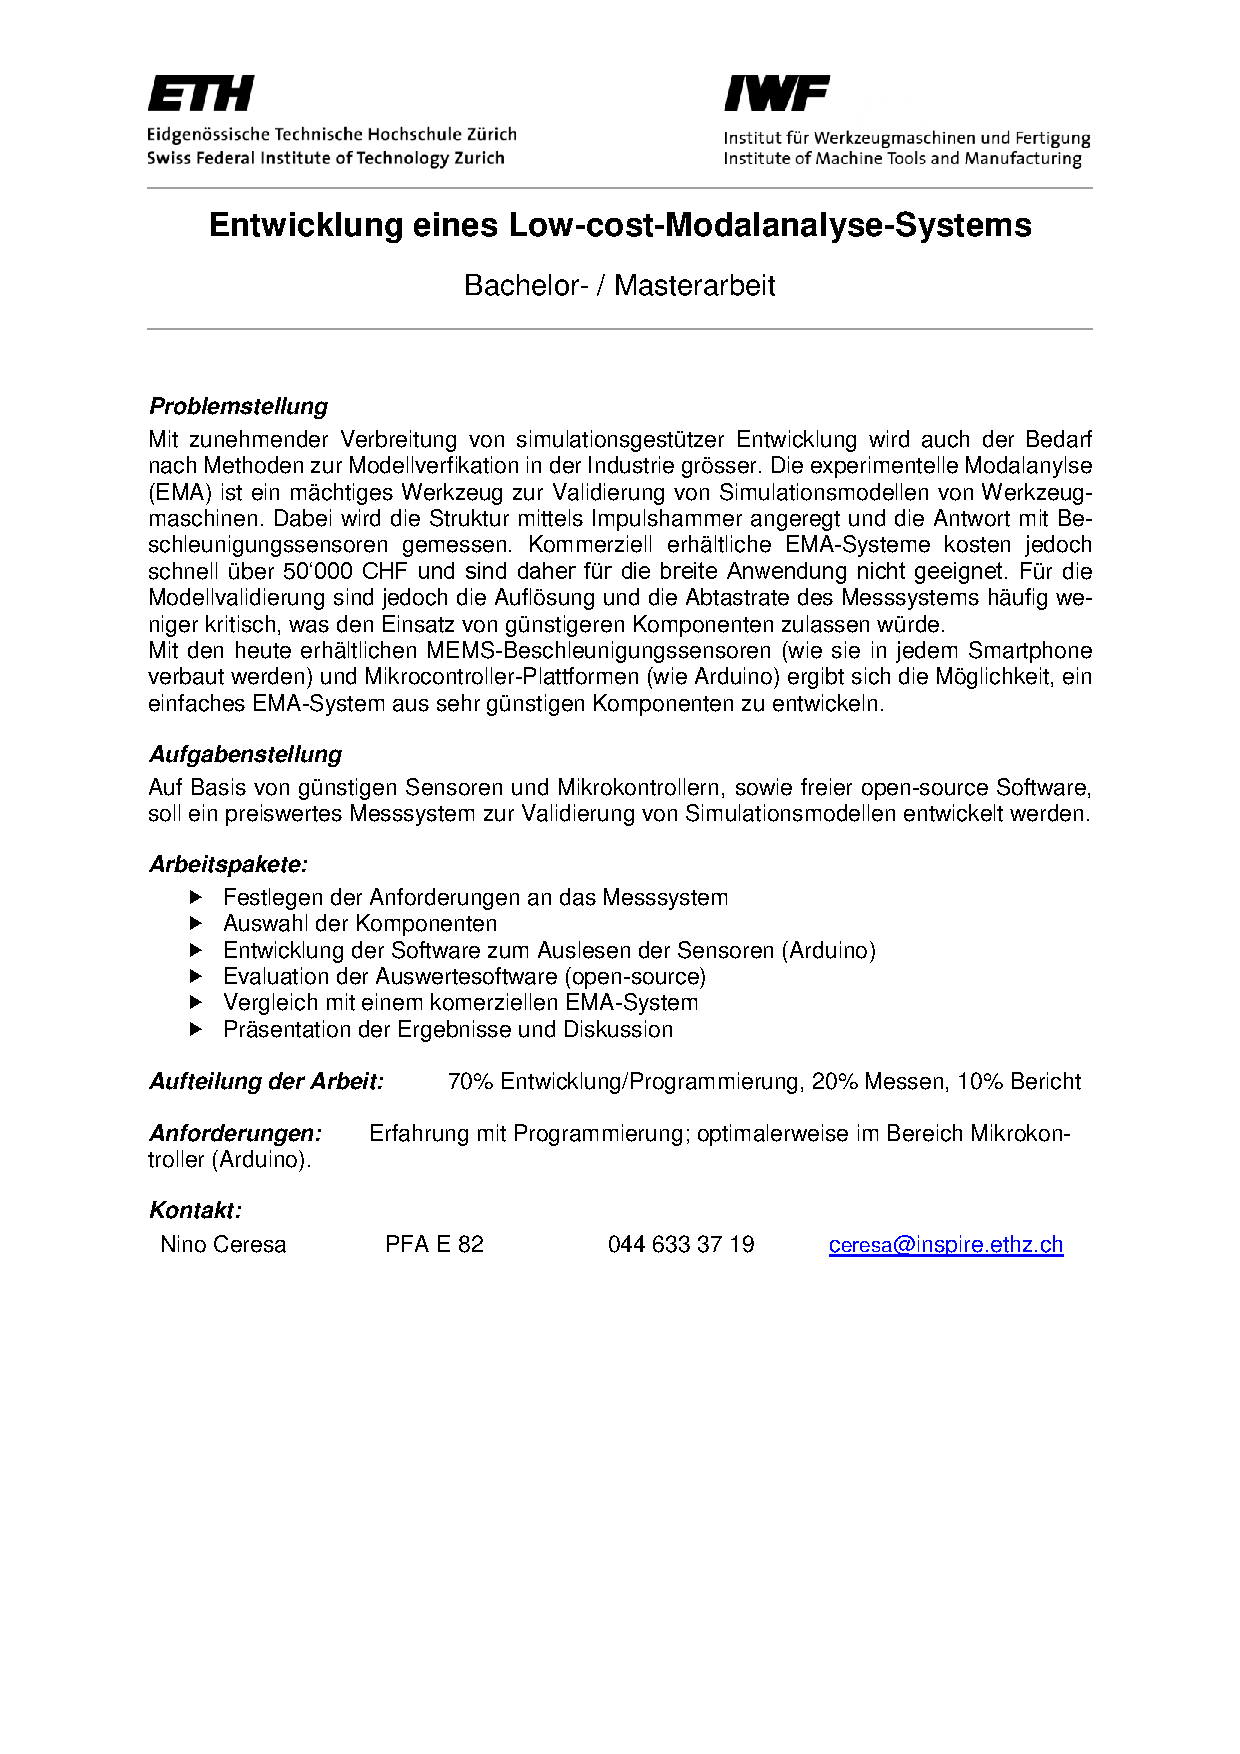
\includepdf{\texpath/task_description.pdf}
\cleardoublepage
\include{\texpath/acknowledgement}

\tableofcontents
\cleardoublepage
%\include{\texpath/symbol}
\chapter*{List of Abbreviations}

\begin{acronym}[ESEVNEI] % Put the longest abbreviation in the square brackets for proper alignment
	\acro{AAF}{Anti Aliasing Filter}
	\acro{ADC}{Analog to Digital Converter}
	\acro{ASCII}{American Standard Code For Information Interchange}
  \acro{CMR}{Common-Mode Rejection}
	\acro{CPU}{Central Processing Unit}
	\acro{DAC}{Data Acquisition}
  \acro{DC}{Direct Current}
	\acro{EMA}{Experimental Modal Analysis}
	\acro{FFT}{Fast Fourier Transform}
	\acro{FIFO}{First In, First Out}
	\acro{FPGA}{Field Programmable Gate Array}
	\acro{FRF}{Frequency Response Function}
  \acro{FT}{Fourier Transform}
	\acro{MCU}{Microcontroller Unit}
	\acro{MEMS}{Micro-Electro-Mechanical-Systems}
  \acro{MISO}{Master In Slave Out}
  \acro{MOSI}{Master Out Slave In}
	\acro{MT}{Machine Tools}
	\acro{LC}{Load Cell}
	\acro{LPF}{Lowpass Filter}
	\acro{LSB}{Least Significant Bit}
	\acro{OPA}{Operational Amplifier}
  \acro{OSI}{Open Systems Interconnection}
  \acro{I2C}[I\textsuperscript{2}C]{Inter-Integrated Circuit}
	\acro{PCB}{Printed Circuit Board}
	\acro{IC}{Integrated Circuit}
	\acro{RS}{Recommended Standard}
  \acro{SAR}{Successive-Approximation}
  \acro{SCLK}{Serial Clock}
  \acro{SNR}{Signal-To-Noise-Ratio}
	\acro{SPI}{Serial Peripheral Interface}
  \acro{SS}{Slave Select}
	\acro{TF}{Transfer Function}
  \acro{UART}{Universal Asynchronous Receiver-Transmitter}
	\acro{USB}{Universal Serial Bus}
	\acro{WLAN}{Wireless Local Area Network}
\end{acronym}

\cleardoublepage

%%%----------------------------------------------------------------
%%% MAIN CONTENT
\mainmatter
\pagestyle{standardheadings}
% set counter to n-1:
\setcounter{chapter}{0}

\chapter{Introduction}

%-----------------------------------------------------
\section{Motivation}
Motivate your work here. 


%-----------------------------------------------------
\section{Related Work}
Previously, this and that has been done and so on.


%-----------------------------------------------------
\section{Overview}
We will first give background information bla bla bla.

% add your chapter files here!
\chapter{State of the Art%
  \label{chap:\currfilebase}}

\section{Measurement}
The process of measurement is the comparison of data from the physical world in the frame of an agreed standard. It is carried out by using an instrument.

This section points to some key aspects of measurement instruments and components, used in the frame of this thesis. As a result some sections of~\cite{webster2018measurement} are summarized.

\subsection{Measurement and Instrumentation}
Measurement instruments translate signals from the physical world into an agreed upon standard. These standardized signals can be compared, altered and stored.
The original data acquired from the physical signal is usually in analog form. This is then converted to digital before it is passed on. The signal chain of a typical digital measurement instrument is shown in \figref{fig:digital_instrument}.

\begin{figure}[!htb]
  \centering
  \includestandalone[width=\linewidth]{figures/measurement/digital_instrument/digital_instrument}
  \caption[Digital Instrument]{Digital measurement instrument%
    \label{fig:digital_instrument}}
\end{figure}

\section{Sensors and Transducers}
A device that responds to a changing phenomenon is called sensor. If we need to transfer from one energy from to another, we use a device called transducer. If one compares sensors and transducers based on the energy input and output, one identifies three types:
\begin{itemize}
  \item In \emph{modifiers} a specific energy form is not converted but modified. Hence they use the same form of energy as input and output.
  \item \emph{Self-generators} give out electric signals from non-electric inputs without the need of additional energy.
  \item \emph{Modulators} in contrast give out electric signals from non-electric inputs, but require an additional energy input.
\end{itemize}

As part of this we focus on self-generating piezoelectric sensors, capacitive modulators that convert mechanical deformation in a static electric field into an electric current, as well as strain gauge based modulators.

\subsection{Sensor Types}

Here we separate different sensors depending on physical value they respond to. In \ac{EMA} we use a force input signal and measure a acceleration, velocity or displacement output signal. Where force is generally detected using Load Cells (\acs{LC}s), the output signal is commonly detected by accelerometers at predefined point on the \ac{MT}. But other setups may be used. Optical methods, for example, allow the detection of the output signal in a non-contacting manner and are preferred when testing very small structures. But for this thesis an approach with low-cost accelerometers is chosen. Therefore, a brief introduction to load cells and accelerometers is given. More on sensor types can be found in \cite{webster2018measurement}.

\subsubsection{Load Cells}

A force measurement sensor that converts a force into an electrical signal is called \acf{LC}. The basis of force measurement results from the physical behavior of a body under external forces. Depending on the bandwidth and magnitude of the signal, as well as the duration of the signal capture, different methods of force measurement are applied in various designs. The methods in brief are \cite{webster2018measurement}:

\begin{itemize}
  \item Balancing the unknown force against a standard mass through a system of levers
  \item Measuring the acceleration of a known mass
  \item Equalizing it to a magnetic force generated by the interaction of a current-carrying coil and a magnet
  \item Distributing the force on a specific area and then measuring the pressure
  \item Converting the applied force into the deformation of an elastic element
\end{itemize}

Furthermore, these methods can be combined with different designs of measuring equipment. Each of which addressing two main problems. First, the physical and geometrical constrains by the application of the device and second, the means by which the force can be converted into an electrical signal.

\subsubsection{Accelerometers}

Accelerometers are sensors that convert acceleration into an electrical signal. In order to measure a physical phenomenon we use seismic masses that act on the sensor structure based on their inertia properties. For example, it is the structure in strain gauge based accelerometers that translates the inertia force into a deformation, where capacitive sensor structures may use deformations or relative motions of separate components in an electric field. In piezoelectric accelerometers the seismic mass deforms a piezoelectric material, see \figref{fig:piezo_sensor}. This is the simplest setup of so called seismic accelerometers.
\\[4ex]
\begin{minipage}{\linewidth}
\centering
\begin{minipage}[b]{0.35\textwidth}
  \centering
  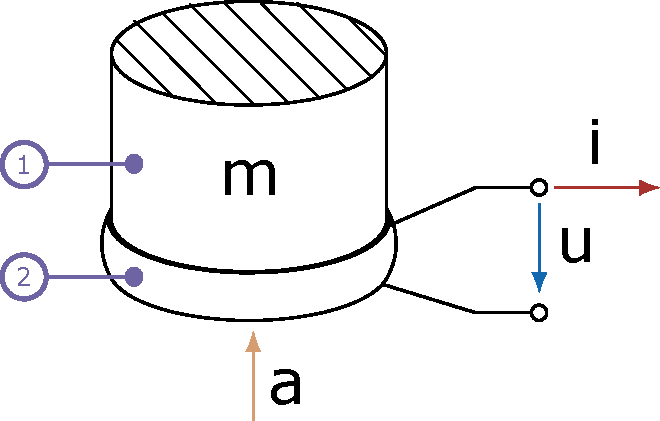
\includegraphics[scale=0.5]{figures/measurement/sensors/piezo_sensor}
  \captionof{figure}[Piezoelectric Accelerometer]{Function principle of a piezoelectric accelerometer%
  \label{fig:piezo_sensor}}
\end{minipage}
\hspace{4em}
\begin{minipage}[b]{0.3\textwidth}
  \centering
  \footnotesize
  \def\circlabel#1#2{%
    \begin{tikzpicture}[%
      x=1em,y=1ex,
      baseline={([yshift=3] N.south)},
      font={\fontsize{6pt}{6.2pt}\selectfont},
      ]%
      \node[%
        circle, fill=white, draw=#1, line width=1pt,
        inner sep=2pt, minimum size=8pt, align=center,
        ] (N) {#2};
      \end{tikzpicture}
  }
  \begin{tabular}{c@{ :\hskip 0.5em}l}
    \toprule
    \large{a} & Acceleration\\
    \large{m} & Mass\\
    \large{i} & Induced Current\\
    \large{v} & Induced voltage\\
    \large{\circlabel{WesMixL8qual3}{1}} & Seismic mass\\
    \large{\circlabel{WesMixL8qual3}{2}} & Piezoelectric material\\
  \bottomrule
  \end{tabular}
  \normalsize
  \captionof{table}[Legend to Piezoelectric Accelerometer]{Legend to \figref{fig:piezo_sensor}%
  \label{tab_piezo_sensor}}
\end{minipage}
\end{minipage}\\[4ex]

In seismic accelerometers the base of the arrangement is motion. When describing the one dimensional case, one can express non-stationary random vibrations acting on the accelerometer as
\begin{align}
  m\dv[2]{z}{t} &= c\dv{z}{t} + kz = mg\cos\pqty{\theta}-m\dv[2]{x_1}{t}
\end{align}
where
\begin{itemize}
  \item $m$ is the seismic mass
  \item $z=x_2-x_1$ is the relative motion between the mass and the base
  \item $x_1$ is the displacement of the base
  \item $x_2$ is the displacement of the mass
  \item $\theta$ is the angle between sense axis and gravity
\end{itemize}
The Laplace transformed second-order system thus takes the form
\begin{align}
  G(s) &= \frac{X(s)}{F(s)} = \frac{K}{s^2/\omega_n^2 + 2\zeta s/\omega_n + 1 \label{eqn:acceler_dynamics}}
\end{align}
where
\begin{itemize}
  \item $s$ is the Laplace operator
  \item $K=1/k$ is the static sensitivity
  \item $\omega_n=\sqrt{k/m}$ is the undamped frequency in \si{\radian\per\second}
  \item $\zeta=c/2\sqrt{km}$ is the damping ratio
\end{itemize}
It is obvious that the performance of accelerometers depends on their static sensitivity, the natural frequency and the damping ratio. We want the accelerometer to have a linear transfer function in the range of operation. But namely the damping ratio can distort a measurement when operating an accelerometer near its eigenfrequency, see \figref{fig:seismic_accelerometer_edited}.
This is the most simplified case, that measures the acceleration in one dimension. In three dimensional accelerometers, that are generally used in \ac{EMA}, the acceleration becomes a function of $\dv*[2]{x}{t}$, $\dv*[2]{y}{t}$ and $\dv*[2]{z}{t}$. Consequently, multiple transducers in multiple channels are used.

\begin{figure}[!htb]
  \centering
  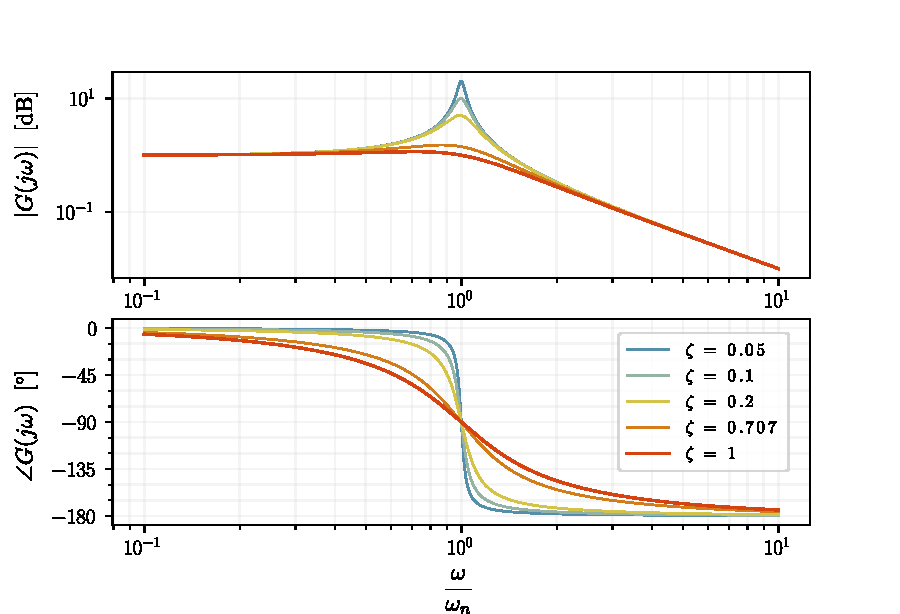
\includegraphics[scale=0.8]{figures/measurement/accel/seismic_accelerometer_edited}
  \caption[Second-Order System Bode Plots]{Bode plots of second order system describing the dynamic behavior of seismic accelerometers%
    \label{fig:seismic_accelerometer_edited}}
\end{figure}

\subsection{Transducer Principles}

The same transducer types can be used in \ac{LC}s and accelerometers due direct relation between acceleration and force in inertial models. Namely in commercially available \ac{EMA}s, piezoelectric transducers are typically used in both the \ac{LC}s and accelerometers. In this section the physical principles of transducers used in this thesis are presented.

\subsubsection{Strain Gauges}

In strain gauge \ac{LC}s and accelerometers the elastic properties of a material probe is exploited.

Given a probe, we apply a controlled load through an external force in \ac{LC}s or through the seismic mass in accelerometers. This load deforms the probe in the elastic region and the deformations are captured by a strain gauge at a suitable location. The probe deformation is proportional to the force acting on the probe because of Hooke's law.

The strain gauges themselves each use a specific length gauge wire in order to reach a resistance of typically \SI{120}{\ohm}. The wire is bonded between two thin sheets in coiled up form as can be seen in \figref{sfig:strain_gauge}. The sheets act as insulating carrier and can be easily deformed with the intent of passing the load to the wire grid. The gauge is attached to the probe structure by a wax or a resin. The intent is that deformations in transversal direction of the strain gauge act on all coils simultaneously, changing their resistance. By using small sized strain gauges with respect to the probe, the mechanical and thermal properties of the strain gauge become negligible small. As an example, we assume the probe expands. Then a strain gauge on its surface experiences tension. The coils in the grid are therefore stretched and as a result of the generalized Hook's law the coil cross sections decrease. Both the strain in axial direction of the coil and the decreased coil cross sections increase the wire's resistance.

In order to measure deformations one needs to take environmental influences into consideration. It is well known that resistance is susceptible to variations in temperature. Placing the strain gauge in a wheatstone bridge, with resistors, that change their resistance in the same manner as the strain gauge will reduce the influence of temperature significantly --- see \figref{sfig:wheatstone_bridge_single}.

\begin{figure}[!htb]
  \centering
  \subcaptionbox{Strain gauge on structure, with (1) Structure, (2) Metal Pad, (3) Grid and (4) Carrier\label{sfig:strain_gauge}}{%
    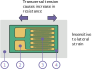
\includegraphics[scale=0.7]{figures/measurement/sensors/strain_gauge}}
  \hspace{4em}
  \subcaptionbox{Strain gauge in Wheatstone bridge circuit\label{sfig:wheatstone_bridge_single}}{%
    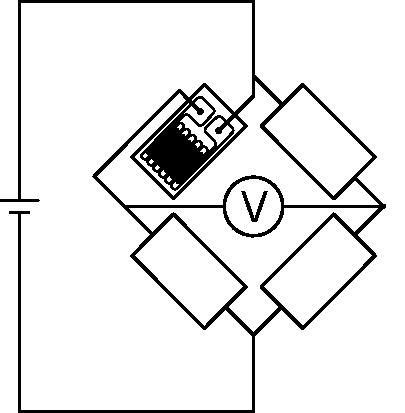
\includegraphics[scale=0.7]{figures/measurement/sensors/wheatstone_bridge_single}}
  \caption[Strain Gauge]{Strain gauge%
    \label{fig:strain_gauge}}
\end{figure}

\subsubsection{Piezoelectric Materials}
Some materials develop electric charge proportional to directly applied mechanical stress. The same materials show the converse effect. A proportional strain of the material will occur to an applied electric field.

The first phenomenon has found its application in a variety of self-generating sensors that output electrical signals, namely in \ac{LC}s and accelerometers, where the piezoelectric charge is converted into a current or voltage signal.

Piezoelectric sensors are designed to exploit the piezoelectric effect of the material in one axis. Additionally, we use amplifier circuits so that the weak electrical signal, induced due to the piezoelectric charge, is elevated to amplitudes that are in the range of operation of standard electronic components. These circuits require additional energy. Commercially available \ac{LC}s therefore require supplied energy, see \figref{fig:piezo_ampcirc}.

\begin{figure}[!htb]
  \centering
  \subcaptionbox{Piezoelectric sensor connected to a voltage amplifier\label{sfig:piezo_voltage_amp}}{%
    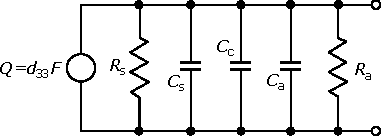
\includegraphics[scale=0.9]{figures/measurement/sensors/piezo_voltage_amp}}
  \hspace{4em}
  \subcaptionbox{Strain gauge in Wheatstone bridge circuit\label{sfig:piezo_current_amp}}{%
    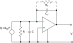
\includegraphics[scale=0.9]{figures/measurement/sensors/piezo_current_amp}}
  \caption[Piezoelectric Sensors in Amplifier Circuits]{Piezoelectric sensors connected to amplifier circuits~\cite{webster2018measurement}%
    \label{fig:piezo_ampcirc}}
\end{figure}

Depending on the design of the sensor, piezoelectric materials are used in different shapes. \figref{fig:piezo_designs} shows some possible variations.


\subsubsection{Capacitive Transducers}

In capacitive transducers the electric field of a capacitor is used as reference. Changes in the electric field of a sensing capacitor generate an electrical signal output at the surrounding circuit. That is, if we change the supply voltage or capacitance of said capacitor, the signal output is non-zero. This gives a broad framework of different transducers that normally use charge-discharge or constant input signals, which enable us to measure either the capacitance or the change in capacitance. The simplest capacitor design consists of two parallel electrodes with capacitance C.
\begin{align}
  C &= f(d,A,\varepsilon)
\end{align}

With variable distance, dielectric material or area and with the measurement of the capacitance, we can then deduce the plate displacement in normal and parallel direction to the plates depending on the method used, see \figref{fig:cap_disp}. In the following some models of the capacitance from \cite{webster2018measurement} are shown.

In \emph{variable displacement} transducers, the distance between two capacitive plates is inversely proportional to the capacitance.
\begin{align}
  C(x) &= \frac{\varepsilon A}{x} = \frac{\varepsilon_r\varepsilon_0 A}{x}
\end{align}
where
\begin{itemize}
  \item $\varepsilon$ is dielectric constant or permittivity
  \item $\varepsilon_r$ is the relative dielectric constant (in air and vacuum $\varepsilon_r\approx 1$)
  \item $\varepsilon_0$ is \SI{8.854188}{\farad\per\meter}, the dielectric constant of vacuum
  \item $x$ is the distance of the plates in \si{\meter}
  \item $A$ is the effective area of the plates in \si{\meter\squared}
\end{itemize}

In \emph{variable area displacement} transducers, the capacitance is proportional to the reduction of area due to the movement of the plate.
\begin{align}
  C(x) &= \frac{\varepsilon_r\varepsilon_0\pqty{A-wx}}{d}\label{eqn:var_ar_displace}
\end{align}
where
\begin{itemize}
  \item $\varepsilon_2$ is the permittivity of the displacing material (e.g.\ liquid)
  \item $w$ is the width
  \item $wx$ is the reduction in the area due to movement of the plate
  \item $d$ is the distance of the plates in \si{\meter}
\end{itemize}

In \emph{variable dielectric} transducers, the capacitance depends on the ratio of each permittivity in the electric field.
\begin{align}
  C(x) &= \varepsilon_0 w \bqty{\varepsilon_2 l - \pqty{\varepsilon_2-\varepsilon_1}x}\label{eqn:var_diel_displace}
\end{align}
where
\begin{itemize}
  \item $x$ is the displacement normal to the plate's direction
  \item $\varepsilon_1$ is the relative permittivity of the dielectric material
  \item $\varepsilon_2$ is the permittivity of the displacing material (e.g.\ liquid)
\end{itemize}

\emph{Differential displacement} sensors are setup in capacitive arrangements that aim to eliminate nonlinearities. Different variations of these types of sensors exist. For example we can allow the outer plates to move and fix the middle one or we can reverse this setup. But the range is equal to twice the separation in both cases.
\begin{align*}
  2\delta C = C_1-C_2 &= \frac{\varepsilon_r\varepsilon_0 lw}{d-\delta d} - \frac{\varepsilon_r\varepsilon_0 lw}{d+\delta d} = \frac{2\varepsilon_r\varepsilon_0 lwd}{d^2+\delta d^2}\\
  C_1+C_2 &= \frac{\varepsilon_r\varepsilon_0 lw}{d-\delta d} + \frac{\varepsilon_r\varepsilon_0 lw}{d+\delta d} = \frac{2\varepsilon_r\varepsilon_0 lwd}{d^2+\delta d^2}\\
\end{align*}
Giving approximately
\begin{align}
  \frac{\delta C}{C} = \frac{\delta d}{d}
\end{align}

\begin{figure}[!htb]
  \sbox0{\subcaptionbox{Variable distance displacement\label{sfig:cap_var_disp}}{%
    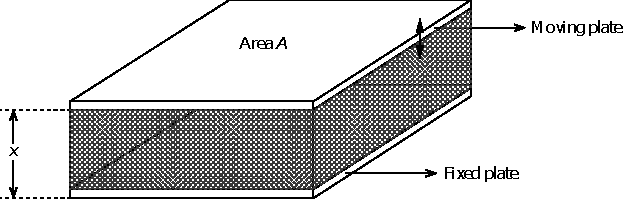
\includegraphics[scale=0.7]{figures/measurement/capac/cap_var_disp}
    }}% a
  \sbox1{\subcaptionbox{Variable area displacement\label{sfig:cap_var_area}}{%
    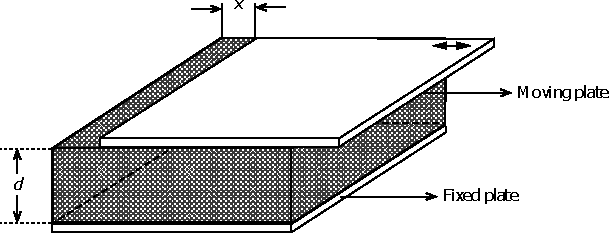
\includegraphics[scale=0.7]{figures/measurement/capac/cap_var_area}
    }}% b
  \sbox2{\subcaptionbox{Variable dielectric displacement\label{sfig:cap_var_diel}}{%
    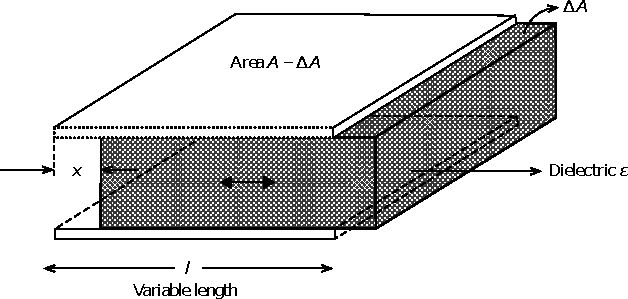
\includegraphics[scale=0.7]{figures/measurement/capac/cap_var_diel}
    }}% c
  \sbox3{\subcaptionbox{Differential capacitive displacement\label{sfig:cap_diff}}{%
    \includegraphics[scale=0.7]{figures/measurement/capac/cap_diff}
    }}% d
  \sbox4{\subcaptionbox{IC smart capacitive displacement \label{sfig:cap_smart}}{%
    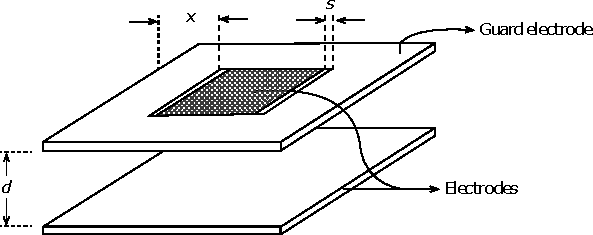
\includegraphics[scale=0.7]{figures/measurement/capac/cap_smart}
    }}% e
  \centering
  {%
    \renewcommand{\arraystretch}{6}%
    \setlength{\tabcolsep}{0em}
    \begin{tabular}{ccc}
      \usebox0 & \usebox1 \\
      \usebox2 & \usebox3 \\
    \end{tabular}%\\[4ex]
    % \usebox4
  }
  \caption[Capacitive Displacement Transducers]{Capacitive displacement transducers \cite{webster2018measurement}%
    \label{fig:cap_disp}}
\end{figure}

Given a sensor design, one can then map the displacement of the respective transducer to the load acting on a \ac{LC}, respectively, when using a seismic mass and the corresponding equation of motion, to the acceleration measured by an accelerometer. The capacitive displacement transducer is applicable for many sensor applications and the fact, that the sensing conductors can be built from a variety of materials and can be optimized for different input voltage levels, makes its form factor scalable in both directions. In a sensor \ac{IC} package, the capacitive transducers can be realized in a smaller form factor or with higher precision at the same size compared to resistive sensors, like strain gauges. A simplified model of the mechanics inside a capacitive \ac{MEMS} sensor are shown in \figref{fig:accelerometer_bent}.

\begin{figure}[!htb]
  \centering
  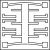
\includegraphics[scale=0.7]{figures/measurement/sensors/accelerometer_bent}
  \caption[Capacitive MEMS Accelerometer]{Capacitive MEMS accelerometer, with acceleration a and the seismic mass m. The bridges attached to the seismic mass act as dielectricum.%
    \label{fig:accelerometer_bent}}
\end{figure}

\section{Signal Conditioning and Processing\label{signal_conditioning_processing}}
In an ideal world, the signal output of a sensor would correlate to the measurand exactly. In real systems this is not the case because of a variety of reasons. In low-frequency applications, the most important ones are:

\begin{itemize}
  \item The voltage or current rating at a sensor's output is not perfectly linear with respect to the measurand. Often the output is pseudo-linear in a limited range of values and deviates from the trajectory for values outside of this range.
  \item Noise and shifts introduced through the inherent impedances of analog components lead to deviations from the voltage or current rating of the sensor as well as deviations of these ratings with respect to the measurand itself.
  \item The quantization process causes the captured value space to have a finite resolution.
  \item Analog signals can only be digitized with a finite sampling rate. A discrete set of data points is captured instead of a continuous signal.
\end{itemize}

The field of signal processing includes analyzing, modifying and synthesizing signals. Most prominently, in data acquisition systems we convert analog signals to digital ones that can be further processed without the parasitic effects of the analog realm. On the opposite side when addressing these parasitic effects one needs to apply signal conditioning. In other words, before every processing step of an analog signal we need to consider signal conditioning. When dealing with digital signals, no signal conditioning is required.

\section{Experimental Modal Analysis}

\ac{EMA} is a powerful tool to detect vibration related problems of mechanical structures. We use modes to characterize resonant vibrations of the system. This section is only a short excerpt of an introduction to \ac{EMA}. An overview has been presented by \citeauthor{schwarz1999experimental} in~\cite{schwarz1999experimental}.

\subsubsection{Vibration}

In every vibration one can observe a combination of two different types of vibrations. The forced and the resonant ones. Forced vibrations in a structure are caused by
\begin{itemize}
  \item Internally generated forces
  \item Unbalances
  \item External loads
  \item Ambient excitations
\end{itemize}
Common examples of vibration sources in \ac{MT} are displayed in \figref{fig:vibration_sources}.

\begin{figure}[!htb]
  \centering
  \subcaptionbox{Axis Motion\label{sfig:ball_screw_simple}}{%
    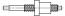
\includegraphics[scale=0.7]{figures/ema/vibration_sources/ball_screw_simple}}
    \hspace{4em}
  \subcaptionbox{Imbalance\label{sfig:imbalance_scheme}}{%
    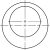
\includegraphics[scale=0.7]{figures/ema/vibration_sources/imbalance_scheme}}
  \hspace{4em}
  \subcaptionbox{Processing Force\label{sfig:processing_force_scheme}}{%
    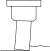
\includegraphics[scale=0.7]{figures/ema/vibration_sources/processing_force_scheme}}
  \\[5ex]
  \begingroup
  \subcaptionbox{Impact Hammer\label{sfig:impulse_hammer_scheme}}[0.5\linewidth]{%
    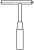
\includegraphics[scale=0.7]{figures/ema/vibration_sources/impulse_hammer_scheme}}
  \endgroup
  \hspace{0em}
  \subcaptionbox{Modal Shaker\label{sfig:modalShaker_scheme}}{%
    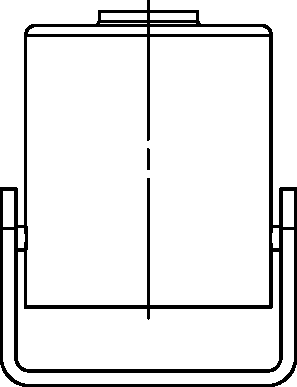
\includegraphics[scale=0.7]{figures/ema/vibration_sources/modalShaker_scheme}}
  \caption[Forced Vibration Sources]{Sources of forced vibration. Note that \subref{sfig:ball_screw_simple}, \subref{sfig:imbalance_scheme} and \subref{sfig:processing_force_scheme} occur during \ac{MT} operation, while \subref{sfig:impulse_hammer_scheme} and \subref{sfig:modalShaker_scheme} are devices that are explicitly used for \ac{EMA} to introduce vibrations into the structure of investigation.%
    \label{fig:vibration_sources}}
\end{figure}

Resonant vibration arises when one or more of the natural modes of vibration, inherent properties of the structure under investigation, is excited. Resonant vibration typically amplifies the vibration response to a level that exceeds deflection, stress and strain caused by static loading.

\subsection{Frequency Response Measurement}

In an \ac{EMA} one needs to determine the \ac{FRF} from input to output. To achieve this we measure the so called response or output function of the structure under investigation. The measurement instrument for this task uses a signal chain in form of \ref{fig:measurement}.
\begin{itemize}
  \item The sensor on the structure translates the physical value (acceleration, velocity or position) into an electrical voltage or current, the analog signal variable.
  \item The amplifier amplifies the typically low power signal to fit it to the input range of the \ac{ADC}.
  \item The \ac{ADC} samples and quantizes the analog signal. It is then converted into a digital signal, in which the quantity is expressed in form of a binary code.
  \item The discrete time signal is then stored on the computer memory.
\end{itemize}

\begin{figure}[!htb]
  \centering
  \includestandalone[width=\linewidth]{figures/ema/measurement/measurement}
  \caption[Frequency Response Measurement]{\ac{FRF} measurement setup%
    \label{fig:measurement}}
\end{figure}

\section{Electronic Components}

This section serves as an introduction to the function of selected electronic components and circuits. It does not give a complete overview of the state of the art. For more background on electronics~\cite{Stiny2019AeB}~and~\cite{Tietze2008EC} may be consulted.

Electronic components are divided into two main types; passive and active ones. Where active components are allowed to generate, amplify or oscillate an electrical signal, passive components can only absorb, dissipate or store electric energy.

\subsection{Passive Components}

Because of the increase in digital processing, the number of passive components has decreased drastically in modern electronic circuits. This, in addition to the trend of using more complex devices in favour to multiple simple passive components, has led to a great variety of passive components which are designed with emphasis on reliability.

Typical examples of passive components are:
\begin{itemize}
  \item \emph{Wires} Depending on the mechanical requirements for the wire, it can either be designed with a solid core or a stranded wire core. A wire consisting of multiple smaller diameter conductors shows better flexibility but reduced current-carrying capacity at the same wire diameter. This is because of the smaller overall conductor cross-section of a stranded wire and, when transmitting high frequency signals, a greater power dissipation due to the more prevalent skin effect. Furthermore the simplicity of solid core wires makes them more resistant to corrosion and more suitable to be used in harsh environments.
  \item \emph{Resistors} Depending on the application different types of resistors can be applied. Fixed value resistors, can be used for safety of other components by dissipating heat or reducing to set the current and voltage in combination relative to other devices. Variable resistors change their value due to different physical phenomena. Thermistors show resistances that are highly susceptible to temperature changes, potentiometers resistance is manually tunable and photoresistors show a light dependant resistance, to name a few.
  \item \emph{Capacitors} store energy in form of an electric field. They have many applications, most prominently in filter circuits and as bypass capacitors to reduce smooth out non constant power draws.
  \item \emph{Inductive Devices} Are devices that store energy in form of an electric field. In modern devices coils are less common due to benefits, when realizing the circuit with capacitors instead. But in specialized applications, namely when converting between electrical and mechanical signals, i.e.\ in motors, generators, loudspeakers etc.
  \item \emph{Transformers} transfer electrical energy from circuit to circuit. Step-up transformers increase the voltage of high alternating current, where step-down decrease the voltages in exchange for higher currents.
\end{itemize}
% \subsubsection{Wires}

% Wires connect several electronic components. Ideally no loss or noise is introduced in wires but inductances occur due to the conductor's shape and material properties as well as electric fields, that are either self induced or present due to ambient conditions.

% Depending on the mechanical requirements for the wire, it can either be designed with a solid core or a stranded wire core. A wire consisting of multiple smaller diameter conductors shows better flexibility but reduced current-carrying capacity at the same wire diameter. This is because of the smaller overall conductor cross-section of a stranded wire and, when transmitting high frequency signals, a greater power dissipation due to the more prevalent skin effect. Furthermore the simplicity of solid core wires makes them more resistant to corrosion and more suitable to be used in harsh environments.

% Braided or foil shielding wires are usually used to shield other wires from ambient fields. Shaped as a tube they enclose one or multiple wires acting as a Faraday cage.

% \subsubsection{Resistors}

% Resistors are loads that reduce the current flow and set the voltage levels within a circuit. There are many different types of resistors.

\subsection{Active Components}
Active components enable the control of high energy signals using small input signals. If the control happens to be continuous and proportional to the input signal, the component used is called linear amplifier. Because of their function, active components typically require additional power supply. Most components of this type include doped semiconductors, therefore conservatively passive semiconductor component are categorized in the group of active components as well. Finally, power sources that don not control signals based on small inputs but rather convert other forms of energies into electrical ones, are included in active components too.

\begin{itemize}
  \item \emph{Diodes} are non-linear components with an asymmetrical current-voltage curve. Because of this the diode is directional where, conventionally defined current is only allowed to flow from anode to cathode. Its analogous in a water circuit is a check valve.
  \item \emph{Bipolar transistors} can be used as amplifier or trigger and are based on semiconductors that are doped with both carriers, i.e.\ electrons and holes. Depending on the surrounding one can amplify voltages, currents or powers with bipolar transistors, but the transistor itself is current controlled.
  \item \emph{Field transistors} or uni polar transistor is doped using only one of the two types of carriers compared to the bipolar transistor. They are voltage controlled.
  \item In an \emph{\acf{IC}} a complete circuitry is produced on a carrier material. Multiple consecutive steps of diffusion, oxidation and etching of a semiconductor result in a multi-layered structure. \ac{IC}s come in packages that are a fraction of the size a circuit of classical components would use. For the categoization of those packages one can look at \figref{fig:ic_flowchart}. The use of \ac{IC}s increases reliability and maintainablity and decreases costs, whenever it is possible to replace a conventional circuit.
  \item The \emph{\acf{OPA}} is a multi-stage, high gain and galvanically coupled differential amplifier. Consisting of multiple transistors in an \ac{IC}, the properties of \ac{OPA}s surpass the ones of single transistors in many designs. Namely, higher gains are possible due to the reduction of the amplified noise.
\end{itemize}

\section{Transmission Protocols}

Digital transmission protocols offer established standards for the communication between \ac{IC}s and devices that at least include a processing unit. There exists a plethora of protocols, that address the communication on a range of different levels of abstraction. Theoretically, these levels can be categorized according to the \acl{OPA} model (\acs{OPA} model), but it is obvious that most protocols address issues on multiple levels. Nevertheless, the model is useful when establishing a new network, since all steps, necessary for a successful communication, are best traced in order of the model. The \ac{OPA} model includes seven layers, as seen in \figref{fig:osi_model}.
\begin{enumerate}
  \item The \emph{physical layer} defines the physical form of the data transmission, i.e.\ the mediumm, in which the data is transmitted and the physical connections.
  \item The \emph{data link layer} addresses the transmission conditions and standards, which allow the communication between two or more devices.
  \item In the \emph{network layer} we implement the definitions for the shortest connections, error detection and addressing techniques.
  \item The \emph{transport layer} ensures that all data is transparent and securely transmitted. Its segmented data is used to detect dublicates and missing data.
  \item The \emph{session layer} establishes channels between devices. It manages open connections and synchronization.
  \item It is the \emph{presentation layer}, where one defines the syntax and semantics of the code.
  \item And the \emph{application layer} that provides the protocols and services that are used in applications. This is the data directly available to the end-user.
\end{enumerate}

When dealing with real hardware, the level of abstraction that can be reached will be limited depending on the device. Namely in the communication between \ac{MCU}s the
Different low end communication protocols can be used to communicate between \ac{IC}s. Many smart devices of today use the \acf{I2C}, the \acf{SPI} or both connections to access their registers. With these protocols two respectively, four wires connect two devices over short distances. When the distance increases or the environment gets to noisy, one needs to improve the cable's isolation, insert active signal repeaters, or switch to another transmission standard.
The transmission standard \acs{RS}-485, defines a widely adopted industry standard of differential digital signal transmission. These offer more stable signal transmissions in harsh environments and over long distances with the caveat of using two wires for each signal.
In depth information about data communication protocols is available in the handbook \cite{buchanan2004handbook}
Rs intro \cite{marais2008rs}

\begin{figure}[!htb]
  \centering
  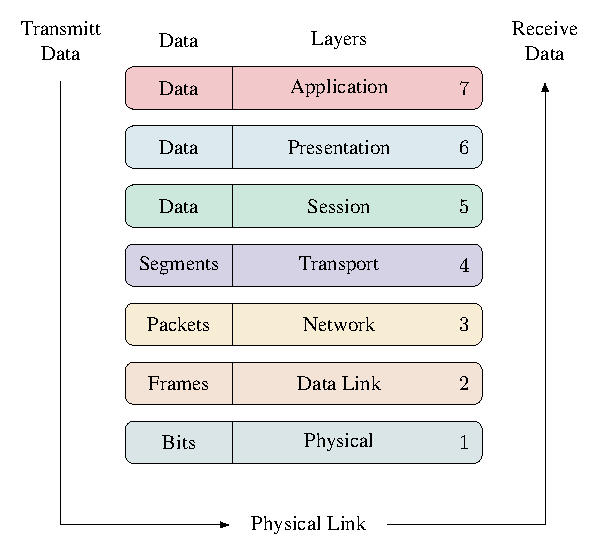
\includegraphics[scale=1]{figures/data_transmission/osi_model/osi_model}
  \caption[OSI Model]{OSI Model%
  \label{fig:osi_model}}
\end{figure}

\subsection{Universal Asynchronous Receiver-Transmitter}
The \ac{UART} protocol is a widely adopted, low-level interface that does not specify the data format or speed. The receiver and transmitter are connected by one wire, that transfers serial bits in form of two voltage-levels, high and low. Both devices must configured to the bit rate for successful signal transmissions. Where the bit rate defines the number of physically transferred bits per second:
\begin{align}
  R_b &= \frac{1}{T_b}
\end{align}
Which is correlated to the baud rate, which defines the transferred symbols in bauds per second (\si{\baud\per\second}):
\begin{align}
  f_{\text{sym}} &= \frac{R}{N}
\end{align}
where the information per pulse $N$ defines the number of bits per pulsed bit. Note that digital systems that use binary code $N=1$ and therefore $f_{\text{sym}}=R_b$.
We often use a two wire setup of \ac{UART} to enable full-duplex transmission between two devices.

\subsubsection{RS-458}
\acs{RS}-485, or EIA-485 is a standard that defines the driver characteristics of a differential serial communication system that has found a wide adoption in industrial control systems. It defines the characteristics of the transmitter and receiver on the physical layer only. Therefore, it does not specify the communication protocol and any serial transmission protocol may be transmitted via this connection. Because it is differential, it uses two channels, labeled A and B, to transmit one signal at a time. In a transmitter the input serial signal is converted two signals of reversed magnitudes. The receiver then reconstructs the original signal by using the difference between the two signals. This is much more reliable than single wire signal, since it can be assumed that all environmental disturbances act on both channels equally, introducing no change to the differential signal between the two. The additional connector C, specified defines the drivers ground.

\subsection{Serial Peripheral Interface}
The \ac{SPI} interface defines a serial connection between two or more devices that requires at least three wires. All transmissions are initiated by a master device, that sends registry addresses as requests. Slave devices, if active, send the data from the requested registry on to the \ac{MISO} wire. The \ac{SCLK} is carrying the master clock, defining the baud rate for all signal transmissions. The \ac{SS} pin activates the slave transmission. A slave can only send and receive if the \ac{SS} pin is activated, which usually means that it is low. This pin can be ignored if only one slave device is present. Because of the naming convention of the data wires, the pins with the same names are connected if one links the master with a slave device. That is \ac{MISO} to \ac{MISO} and \ac{MOSI} to \ac{MOSI}. When daisy chaining multiple slave devices one needs to link the wires with reverse naming, to ensure data transmission in series. In this mode all slave devices are active at the same time and each appends its registry data to the previous ones. The typical bus setups can be seen in \figref{fig:spi_bus}.

\begin{figure}[!htb]
  \centering
  \subcaptionbox{Independent slave configuration\label{sfig:spi_bus_ind}}{%
    \includestandalone[scale=0.72]{figures/data_transmission/spi_bus_ind/spi_bus_ind}}
  \hfill
  \subcaptionbox{Daiy chain configuration\label{sfig:spi_bus_daiy}}{%
    \includestandalone[scale=0.72]{figures/data_transmission/spi_bus_daisy/spi_bus_daisy}}
  \caption[SPI Bus Configurations]{\ac{SPI} bus configurations%
    \label{fig:spi_bus}}
\end{figure}
%\subsubsection{Inter-Integrated Circuits Protocol}

%\subsection{USB}
%\ac{USB}

\chapter{Data Acquisition and Software}
\label{chap:\currfilebase}


\section{Data acquistion}

The \ac{DAC} system developed in this thesis is an open source Arduino based system consisting of multiple microcontrollers. All signal channels are transmitted to a central microcontroller before passing to a computer that serves as visualization and analysis tool.

\begin{figure}[!htb]
    \centering
    \subcaptionbox{Without signal conditioning\label{sfig:dac_comp_simple}}
        {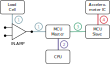
\includegraphics[scale=0.5]{\imgpath/dac/dac_components/dac_comp_simple}}
        \hfill
    \subcaptionbox{With signal conditioning and external \ac{ADC}\label{sfig:dac_comp_precond}}
        {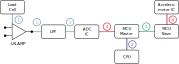
\includegraphics[scale=0.5]{\imgpath/dac/dac_components/dac_comp_precond}}
    \\[0.5em]
    \caption[DAC building blocks]{\acs{DAC}-system building blocks -- note that \ref{sfig:dac_comp_simple} has been realized, but \ref{sfig:dac_comp_precond} has not been implemented yet, due to communication issues between the devices}
    \label{fig:dac_building_blocks}
\end{figure}

\begin{table}[!htb]
    \centering
    \def\linelabel#1#2{%
        \begin{tikzpicture}[%
            x=1em,y=1ex,
            baseline=(N.south),
            font={\fontsize{6pt}{6.2pt}\selectfont},
            ]%
            \draw[#1, line width=1pt] (0,1) -- (1,1) node [
                midway, above, yshift=1,
                circle, fill=white, draw=#1, line width=1pt,
                inner sep=2pt, minimum size=8pt, align=center,
                ] (N) {#2};
        \end{tikzpicture}
    }
    \footnotesize
		\begin{tabular}{c@{ :\hskip 0.5em}l}
            \toprule
            \multicolumn{2}{c}{Interfaces}\\
            \midrule
            \linelabel{WesMixL8qual0}{1} & Analog Signal\\
            \linelabel{WesMixL8qual3}{2} & \ac{USB}\\
            \linelabel{WesMixL8qual4}{3} & \ac{RS}-485\\
            \linelabel{WesMixL8qual6}{4} & \ac{SPI}\\
			\bottomrule
		\end{tabular}
    \normalsize
    \caption[Legend to DAC building blocks]{Legend to \figref{fig:dac_building_blocks}}
\end{table}

\subsection{Building Blocks}

Building blocks are the main components used in the \ac{DAC} signal chain. Additional components that are required to enable the stable operation of the building blocks are not listed.

Because the of accelerometer \ac{IC} output interfaces it is not possible to connect all sensors directly to one \ac{MCU} that acts as a \ac{DAC}. We need to transform the signal to a different interface. A low-cost and versatile method to achieve this, is to use a \ac{MCU} for each accelerometer \ac{IC}. These read the sensor \ac{IC} registers and communicate to the \ac{MCU} master. The master, on the other hand, acts as a passthrough and transmits the data to the \ac{CPU}. In the setup used, it also reads out the \ac{LC} signal. \tabref{tab:mcu_used} lists the \ac{MCU}s used during this thesis.% Other components can be found in \autoref{apx:appendix}.

The analog signal output of the \ac{LC} needs to be amplified to match the input range of the \ac{ADC}. To gain the maximum resolution, this depends on the expected input range. To get a higher value resolution than offered by the \ac{MCU} embedded \ac{ADC} one can set in an external \ac{ADC} \ac{IC} upstream to the \ac{MCU}. Additionally, we use a \ac{LPF} in \figref{sfig:dac_comp_precond}. The \ac{LPF} is needed to cut off high frequency components of the signal that occur particularly in sharp impulse signals. This design choice may lead to problems because it is not standard procedure in the development a measurement instrument. Typically, components in the analog signal chain are chosen, based on the frequency bandwidth of the input signal. This means, the cut-off frequency of the \ac{LPF} is set well above the signal's bandwidth. But because we use low-cost components in our system, the bandwidth is limited to half the sampling rate of the slowest sensor. According to the Nyquist frequency theorem, the cut-off frequency then needs to be reduced to half the sampling frequency, potentially reducing the output magnitude of higher frequency components of the signal.

\begin{table}[!htb]
    \centering
    \def\coltitle#1{\multicolumn{1}{c}{#1}}
    {\renewcommand{\arraystretch}{2.5}%
    \footnotesize
		\begin{tabular}{lcccccc}
            \toprule
            \coltitle{Name} &
            \coltitle{Core} &
            \coltitle{\makecell{\ac{ADC}-Reso-\\lution / \si{bit}}} &
            \coltitle{\makecell{Operating\\Voltage / \si{\volt}}} &
            \coltitle{\makecell{Clock Speed\\ / \si{\mega\hertz}}} &
            \coltitle{\makecell{Flash Me-\\mory / \si{\kilo Byte}}} &
            \coltitle{\makecell{SRAM\\ / \si{\kilo Byte}}}\\
            \midrule
            Arduino Due & \makecell{AT91SAM3\\ARM Cortex} & 12 & 3.3 & 84 & 512 & 96\\
            Teensy 3.2 & \makecell{MK20DX256VLH\\Cortex-M4} & \makecell{13\\ \scriptsize{(\SI{16}{bit}-values)}} & 3.3 & 72 & 256 & 64\\
            \makecell[l]{Robotdyn\\Blackpill} & \makecell{STM32F103C8\\Cortex-M3} & 12 & 72 & 64 & 20\\
            \bottomrule
		\end{tabular}
    \normalsize
    }
    \caption[MCUs used]{List of \ac{MCU}s used in this work}
    \label{tab:mcu_used}
\end{table}


\subsection{Interfaces}

The interfaces are the connections and protocols between the different building blocks of the \ac{DAC} system. The interfaces are chosen based on the sensors used and the expected data rate at the required cable length between each section. I.e.:

\begin{itemize}
    \item Between the analog \ac{LC} and the external \ac{ADC} in \figref{sfig:dac_comp_precond} and the \ac{MCU} integrated \ac{ADC}  in \figref{sfig:dac_comp_simple} respectively the signal transmission is analog.
    \item The register of the accelerometer \ac{IC} is accessed via \ac{SPI}
    \item The communication between \acs{MCU}s is rooted in \acs{RS}-485 differential transmission to accommodate for signal transmission over cable lengths greater than \SI{10}{\meter} and uses a specialized protocol to keep data packages as small as possible.
    \item Between the \ac{MCU} and the \ac{CPU} \ac{USB} transmits data using the serial class of the Arduino software.
\end{itemize}

Data rates and package sizes are critical when sampling at high frequencies. 

With \ac{RS}-485 data can be transmitted over distances of no less than \SI{100}{\km} at a data rate of \SI{1}{\kilo bit\per\second}. At \SI{1200}{\meter} cable length we can reach data rates of around \SI{100}{\kilo bit\per\second}. In our range of application, i.e. a few tens of \si{\meter}, we can expect data rates of \SI{1}{\mega bit\per\second}, thus representing the bottle neck in the digital data chain. If we then transmit \SI{80}{bit} acceleration measurements (see \figref{fig:data_flow}) at \SI{1.6}{\kilo\hertz} we stay below this expected limit by a safety factor of more than 10.
The arduino the serial package parses all data as human readable code, specifically \acf{ASCII}. In this format every digit of integer values is passed as \SI{8}{bit}-value. Which means that a \SI{32}{bit} timestamp and every single axis acceleration are passed as ten \SI{8}{bit}-values and six \SI{8}{bit}-values respectively. This increases the size of an accelerometer package to \SI{624}{bit}, which in turn reduces the safety factor to approximately 1.
It is clear that one cannot use human readable code to transmit the data and guarantee stability at the required sampling rate.


\subsubsection{MCU communication protocol}

The communication protocol for \ac{MCU} to \ac{MCU} and \ac{MCU} to computer was developed for this project.

\begin{table}[!htb]
    \centering
    \includestandalone[scale=1]{\imgpath/software/mcu_com_protocol/mcu_com_protocol}
    \\[0.5em]
    \footnotesize
		\begin{tabular}{c@{ :\hskip 0.5em}l}
			\toprule
            \large{\textcolor{WesMixL8qual6}{<[}/\textcolor{WesMixL8qual6}{]>}} & Start-/End-bytes, represented as \ac{ASCII}\\
            \textcolor{WesMixL8qual0}{\large (reg)} & Registry/Address of the transmission\\
            \textcolor{WesMixL8qual4}{\large (\#Bytes)} & Number of bytes in transmission\\
            \textcolor{WesMixL8qual5}{\large (data)} & Data to transmit\\
			\bottomrule
		\end{tabular}
	\normalsize
    \caption[MCU communication protocol]{Protocol used to communicate between two MCU's and between MCU and computer}
    \label{tab:mcu_com_protocol}
\end{table}

%     output signal that must be amplified by an \ac{IN-AMP} to scale up the signal to the operating range of the consecutive components.

% . to of smart sensor IC are predetermined. With \ac{SPI}Standard interfaces, determined by senor ic
% MCU com based uart length -> differential transmission using the rs-485 protocol, introduces slave master com, only one slave can speak at a time



\subsection{Dataflow}

All \acs{MCU}s operate sequentially.
The dataflow in \ac{MCU} must be sequential. For this reason during a measurement all data is passed to a central \ac{MCU}, where it is streamlined to the pc. The central \ac{MCU} or master cycles through all connected \ac{MCU} performing a data request, hold and receive action. As soon as a slave \ac{MCU} gets a request, it transmits a data package from its buffer. The master now receiving the data package will throughput the signal to the \ac{CPU}, where it is stored. By the end of this process the master will jump to the next slave.

All measurements consist of a \SI{32}{bit}-timestamp and the measured values and are pushed into a \ac{FIFO} buffer in the flash memory of the \ac{MCU}, directly connected to the sensor. Bundled data packages are then pulled from the buffer and translated into the transmission code as defined in \tabref{tab:mcu_com_protocol}. In \figref{fig:data_flow} the data flow is represented by a system that is using only one slave \ac{MCU}, displayed in violet.

Measurements are packaged due to the time the master requires to change the communication to another slave. During these switches no data is transmitted eventually bottlenecking the data rate of the system.

\begin{figure}[!htb]
    \centering
    \includestandalone[width=0.8\linewidth]{\imgpath/software/data_flow/data_flow}
    \caption[Data flow]{Data flow between two \ac{MCU}s and the CPU}
    \label{fig:data_flow}
\end{figure}

\section{Software}

The software developed during this project is split into the Arduino software running on the \acs{MCU}s and a python based tool to receive and visualize the data via \ac{USB}.

For the instrument to work, some functions are required, while other desired functions are tools that simplify the workflow during measurements and facilitate bug fixes in the software.

The requirements to the software tools are:
\begin{enumerate}[label=\emph{m\arabic*}, itemindent=3em, labelsep=2em]
    \item Read out accelerometer and \ac{LC} data at the maximum sample speed of the accelerometer \ac{IC}.\label{req:read_out}
    \item Synchronize measurements timestamps.\label{req:sync}
    \item Initialize measurement by hammer impulse.\label{req:init}
\end{enumerate}

The desired software tools are:
\begin{enumerate}[label=\emph{w\arabic*}, itemindent=3em, labelsep=2em]
    \item Generate continuous real time output of measurement data.\label{des:cont_out}
    \item Track data transfer via \ac{USB}.\label{des:dat_track}
\end{enumerate}

% \subsubsection*{\ref{req:read_out}:}
% The target is to read out data from two or more accelerometer \acs{IC}s and the data from the \ac{LC} in form of the data flow as in \figref{fig:data_flow}.

% values in a \ac{DAC} system with multiple 
\chapter{Test Setups%
  \label{chap:\currfilebase}}

The test conducted during this thesis isolated features of the prototype system described in \chpref{chap:dac_software}. Measurement data has been compared to a reference system, called MODE3. Both systems are configured to include one impulse hammer, one \ac{DAC} system and one three dimensional accelerometer, as well as a read out computer system with accompanying software.

\section{Sensor Comparison}
\subsubsection{Accelerometer}
\begin{table}
  \centering
  {\renewcommand{\arraystretch}{1}%
  \footnotesize
  \begin{tabular}{lcccccc}
    \toprule
    \multicolumn{1}{c}{Accelerometer} & \makecell{in system\\\dots} & \makecell{Sensing\\element} & \makecell{Bandwidth\\/ \si{\hertz}} & \makecell{Dynamic\\range / \si{g}} & \makecell{Acceleration noise\\density / \si{\mu g\per\sqrt\hertz}} & \makecell{Estimated\\ cost / $\mathrm{CHF}$}\\
    \midrule
    PCB-356B18  & MODE3 & Piezoceramic & \SIrange{0.3}{5000}{\relax} & $\pm 5$ & \makecell{1.2\\\scriptsize{(at \SI{100}{\hertz})}} & 2500\\
    LIS3DSH  & Prototype & Capacitive & \SIrange{0}{800}{\relax} & \makecell{$\pm 2/\pm 4/\pm 6/$\\$\pm 8 /\pm 16$ \scriptsize{(selectable)}} & \makecell{150\\\scriptsize{(at \SI{100}{\hertz} and $\pm\SI{2}{g}$)}} & 5\\
    \bottomrule
  \end{tabular}
  \caption[Accelerometer Comparison]{Accelerometer comparison%
    \label{tab:acc_compare}}
  \normalsize
  }
\end{table}

\subsubsection{Load Cell}
\begin{table}
  \centering
  {\renewcommand{\arraystretch}{1}%
  \footnotesize
  \begin{tabular}{lcccccc}
    \toprule
    \multicolumn{1}{c}{\makecell{Load Cell\\with hammer}} & \makecell{in system\\\dots} & \makecell{Sensing\\element} & \makecell{Frequency\\response / \si{\hertz}} & \makecell{Range / \si{\kilo\newton}} & \makecell{Sensitivity\\/ \si{\micro\volt\per\newton}} & \makecell{Estimated\\ cost / $\mathrm{CHF}$}\\
    \midrule
    IEPE Type A2000 & MODE3 & Piezoceramic & 5400 & 20 & 200 & 1800\\
    DYMH-103 with hammer  & Prototype & Strain gauge & unknown & 3 & \SIrange{3.3}{5}{\relax} & 120\\
    \bottomrule
  \end{tabular}
  \caption[Load Cell and Hammer configurations]{\ac{LC} and hammer configurations%
    \label{tab:lc_compare}}
  \normalsize
  }
\end{table}

\section{Hammer-Hammer Test}

The hammer tips of the impact hammers of both the the prototype system and the MODE3 are hit against each other. The target of this test is to evaluate the signal quality of the \ac{LC} in the prototype system.

We assume the force transmission from the point of impact to both load cells respectively to be lossless. Thus the recording accuracy of the prototype system is determined by the correlation of the two signal recordings.

The configurations used in the tests are listen in \tabref{tab:hh_config}. The components are shown in \figref{fig:HH_parts}. All hammer-hammer tests were conducted, using a \ac{DAC} of form \figref{sfig:dac_comp_simple}

\begin{table}
  \centering
  {\renewcommand{\arraystretch}{1}%
  \footnotesize
  \begin{tabular}{lccccc}
    \toprule
    \multicolumn{1}{c}{ADC} & \makecell{in system\\\dots} & \makecell{Number of\\channels} & \makecell{A/D resolution\\/ \si{bit}} & \makecell{Sample rate\\/ \si{S\per\second}} & \makecell{Estimated\\ cost / $\mathrm{CHF}$}\\
    \midrule
    \makecell{FOCUS II\\\scriptsize(Dynamic signal analyzer)} & MODE3 & \makecell{4\\\scriptsize{(differential)}} & 24 & \SIrange{2}{96000}{\relax} & 3000\\
    \makecell{Arduino Due} & Prototype & \makecell{12\\\scriptsize{(single-ended)}} &  12 & \SIrange{0}{1e6}{\relax} & 45\\
    \bottomrule
  \end{tabular}
  \caption[Hammer-Hammer Test Configuration]{Hammer-hammer test configuration%
    \label{tab:adc_compare}}
  \normalsize
  }
\end{table}

%\\[4ex]
\begin{minipage}{\linewidth}
\centering
\begin{minipage}[b]{0.65\textwidth}
  \centering
  \includestandalone[scale=0.7]{figures/test_setups/HH_parts/HH_parts}
  \captionof{figure}[Hammer-Hammer Test components]{Hammer-Hammer test components%
    \label{fig:HH_parts}}
\end{minipage}
\hspace{0em}
\begin{minipage}[b]{0.3\textwidth}
  \centering
  \footnotesize
  \def\circlabel#1#2{%
    \begin{tikzpicture}[%
      x=1em,y=1ex,
      baseline={([yshift=3] N.south)},
      font={\fontsize{6pt}{6.2pt}\selectfont},
      ]%
      \node[%
        circle, fill=white, draw=#1, line width=1pt,
        inner sep=2pt, minimum size=8pt, align=center,
        ] (N) {#2};
    \end{tikzpicture}
  }
  \begin{tabular}{c@{ :\hskip 0.5em}l}
    \toprule
    \large{\circlabel{WesMixL8qual3}{1}} & Piezo + \acs{AMP}\\
    \large{\circlabel{WesMixL8qual3}{2}} & Soft Tip\\
    \large{\circlabel{WesMixL8qual3}{3}} & Tip 34CrMo4\\
    \large{\circlabel{WesMixL8qual3}{4}} & \acs{LC} DYMH-103\\
    \large{\circlabel{WesMixL8qual3}{5}} & \acs{IN-AMP} AD627\\
    \bottomrule
  \end{tabular}
  \normalsize
  \captionof{table}[Legend to Hammer Hammer Test Components]{Legend to \figref{fig:HH_parts}%
    \label{tab:HH_parts}}
\end{minipage}
\end{minipage}\\[4ex]

\section{Andromeda Measurement}

In the Andromeda measurement the accelerometers of both systems are positioned at close locations on the Andromeda test bench. Impact hammers of both the prototype and the reference system may be used as input signal. Because of this, the recording of the accelerometer signal of whichever system's impact hammer is not in use, is initiated before the impact and over a longer time frame. To compare signals of both systems, they are synchronized in the post analysis. The target of this test is to evaluate the signal quality of the accelerometer in the prototype system.

The Andromeda test bench consists of a wagon that is supported by a \SI{3}{\meter} long linear drive in the x-axis on two \SI{2.6}{\meter} apart, gantry y-axes that are linear drives as well. Hence kinematic chain
\begin{align*}
  V[b [Y1 Y2] X]
\end{align*}

\figref{fig:andromeda_pics} shows the test setup, while \figref{fig:andromeda_positions} shows an example position of impact in the test setup.

The focus of this test is to compare the accelerometer signals. Therefore, we set the accelerometer parameter as defined in \tabref{tab:set_acc_par}

\begin{table}[!htb]
\centering
\def\coltitle#1{\multicolumn{1}{c}{#1}}
  {\renewcommand{\arraystretch}{1.5}%
  \footnotesize
  \begin{tabular}{lccc}
    \toprule
    \makecell{Sensor\\Parameter} &
    \makecell{Sample\\Rate / \si{Hz}} &
    \makecell{Dynamic\\Range / \si{g}} & \makecell{Quanti-\\zation / \si{bit}}\\
    \midrule
    Reference & 1600 & $\pm$5 & 24\\
    Prototype & 1600 & $\pm$4 & 16\\
    \bottomrule
  \end{tabular}
  \normalsize
  }
  \caption[Set Accelerometer Parameters]{Accelerometer parameter settings%
    \label{tab:set_acc_par}}
\end{table}

\begin{figure}[!htb]
  \centering
  \subcaptionbox{Andromeda test setup\label{fig:andromeda_pics}}{%
    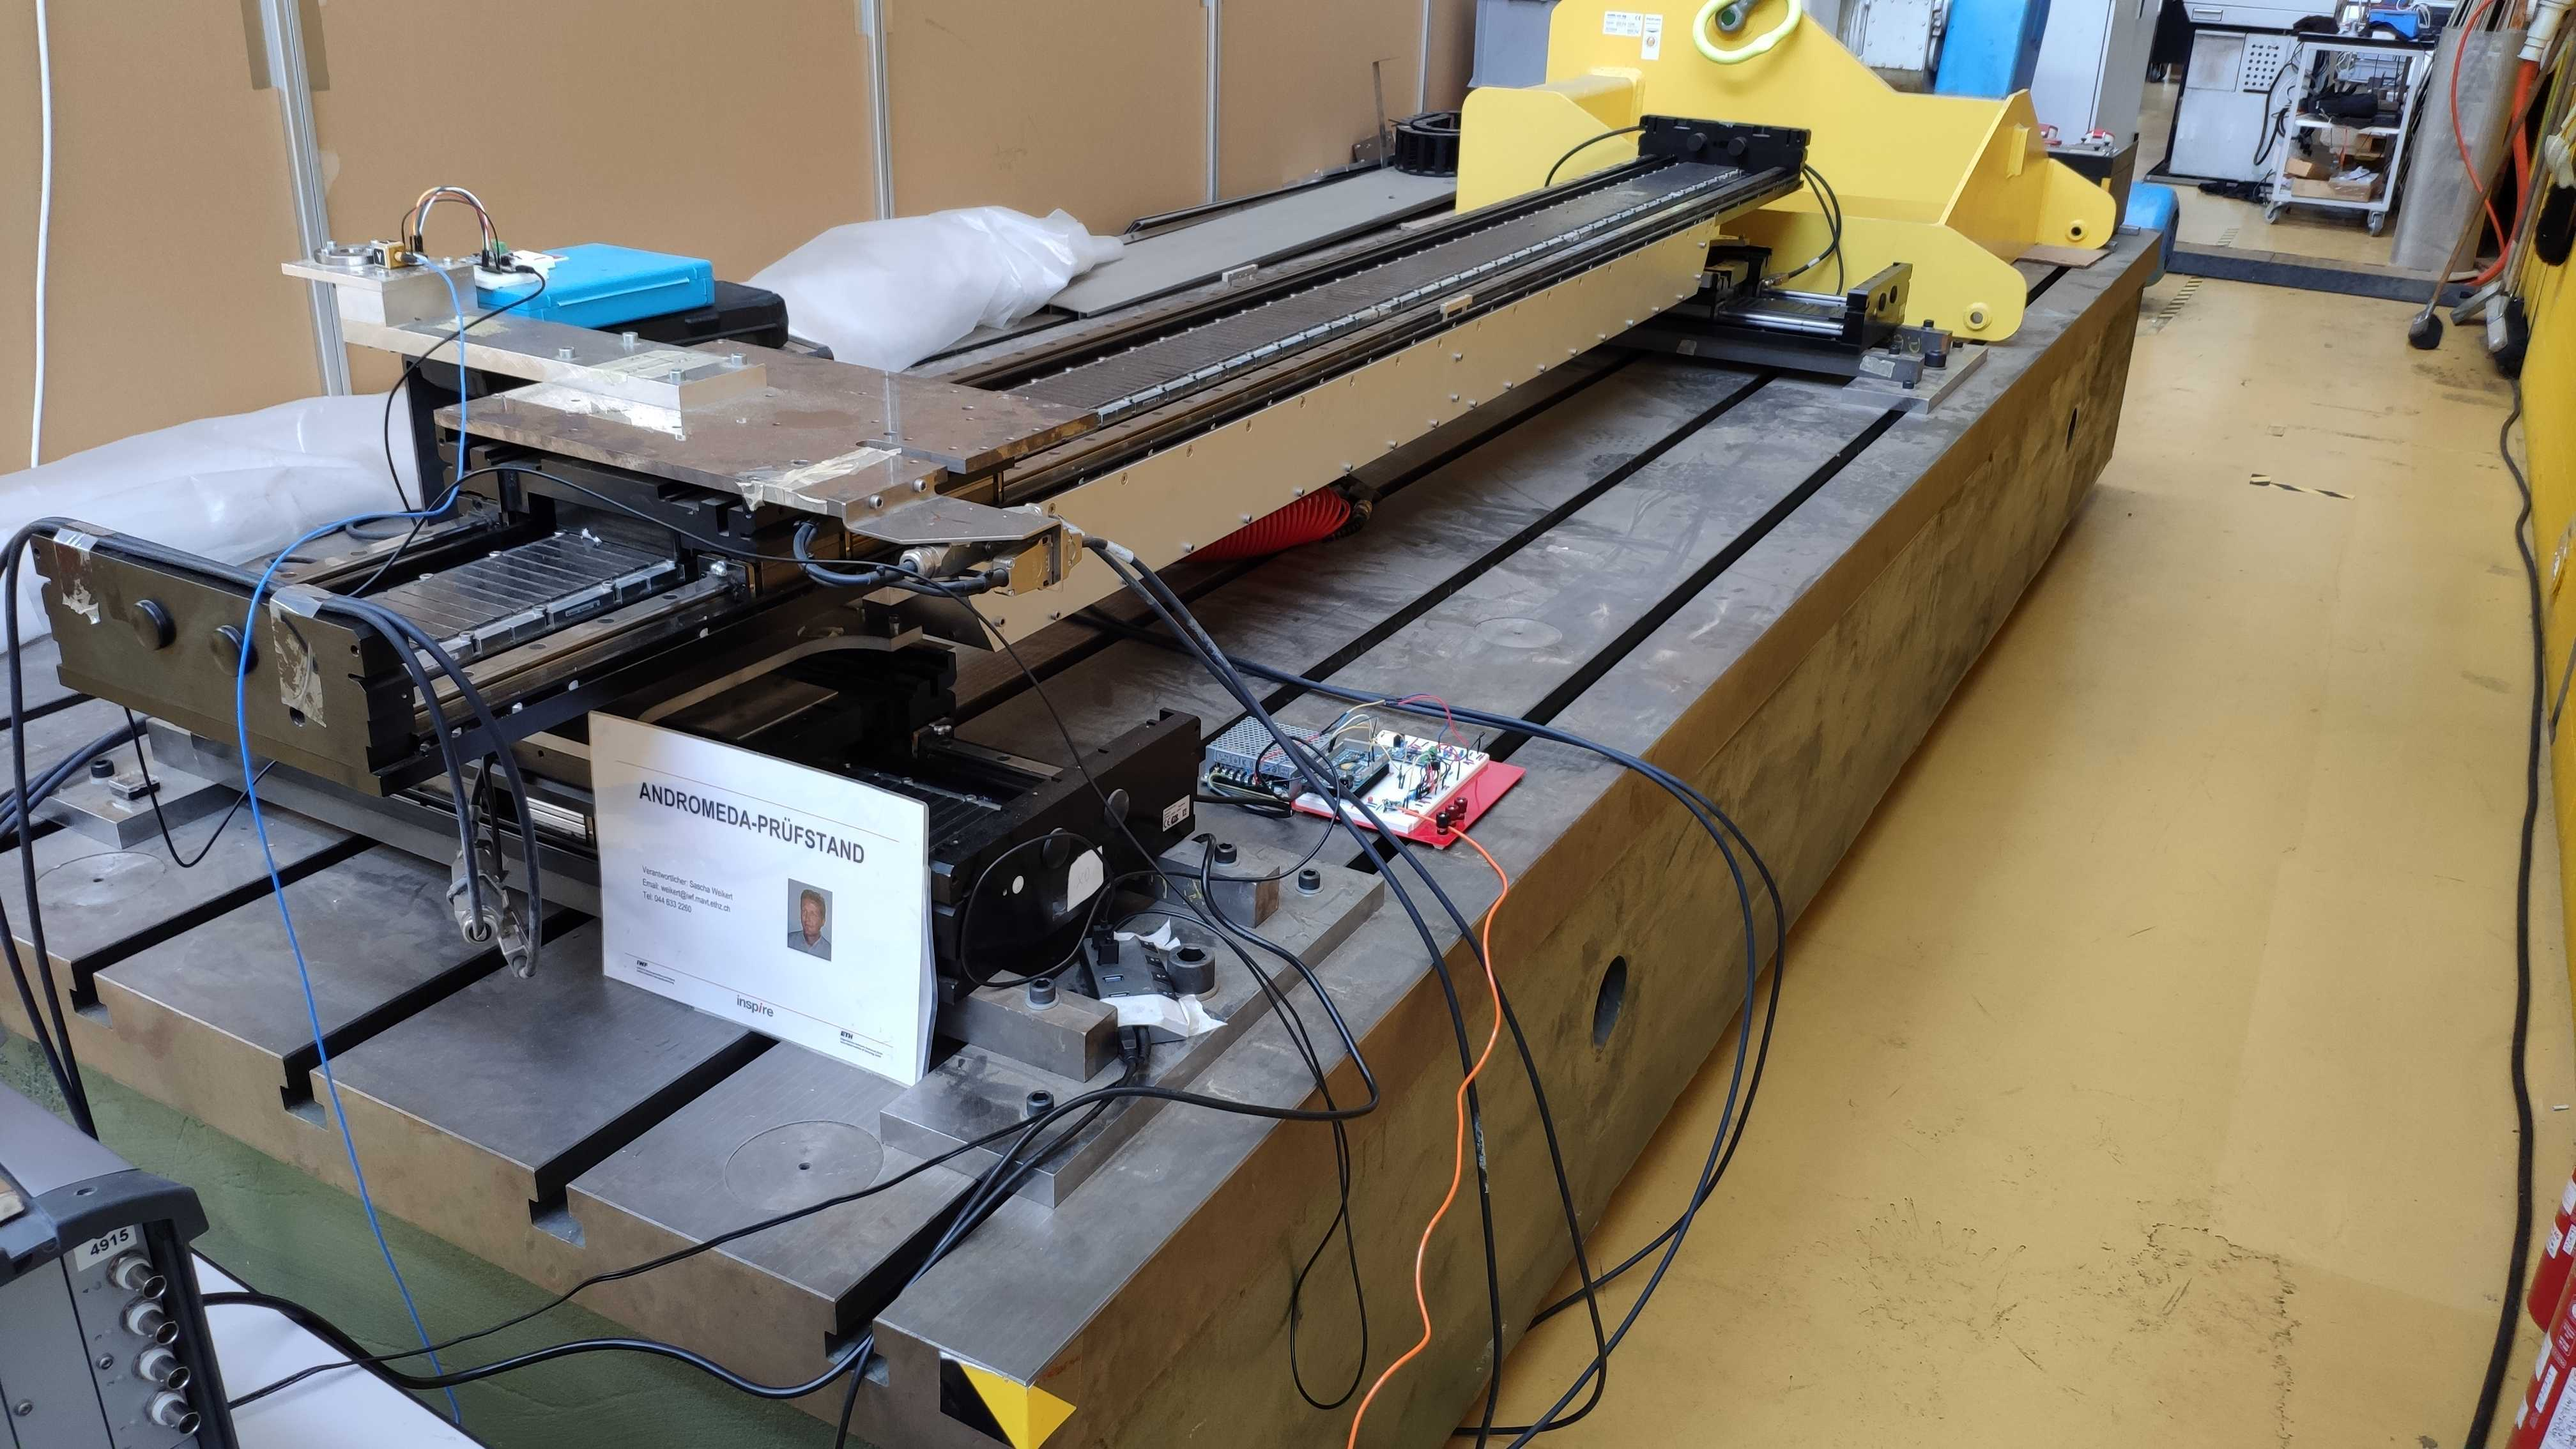
\includegraphics[width=0.50\linewidth]{figures/test_setups/Andromeda/Andromeda_total.jpg}}
    \hspace{4em}
  \subcaptionbox{Acceleromer view\label{sfig:Andromeda_sensors}}{%
    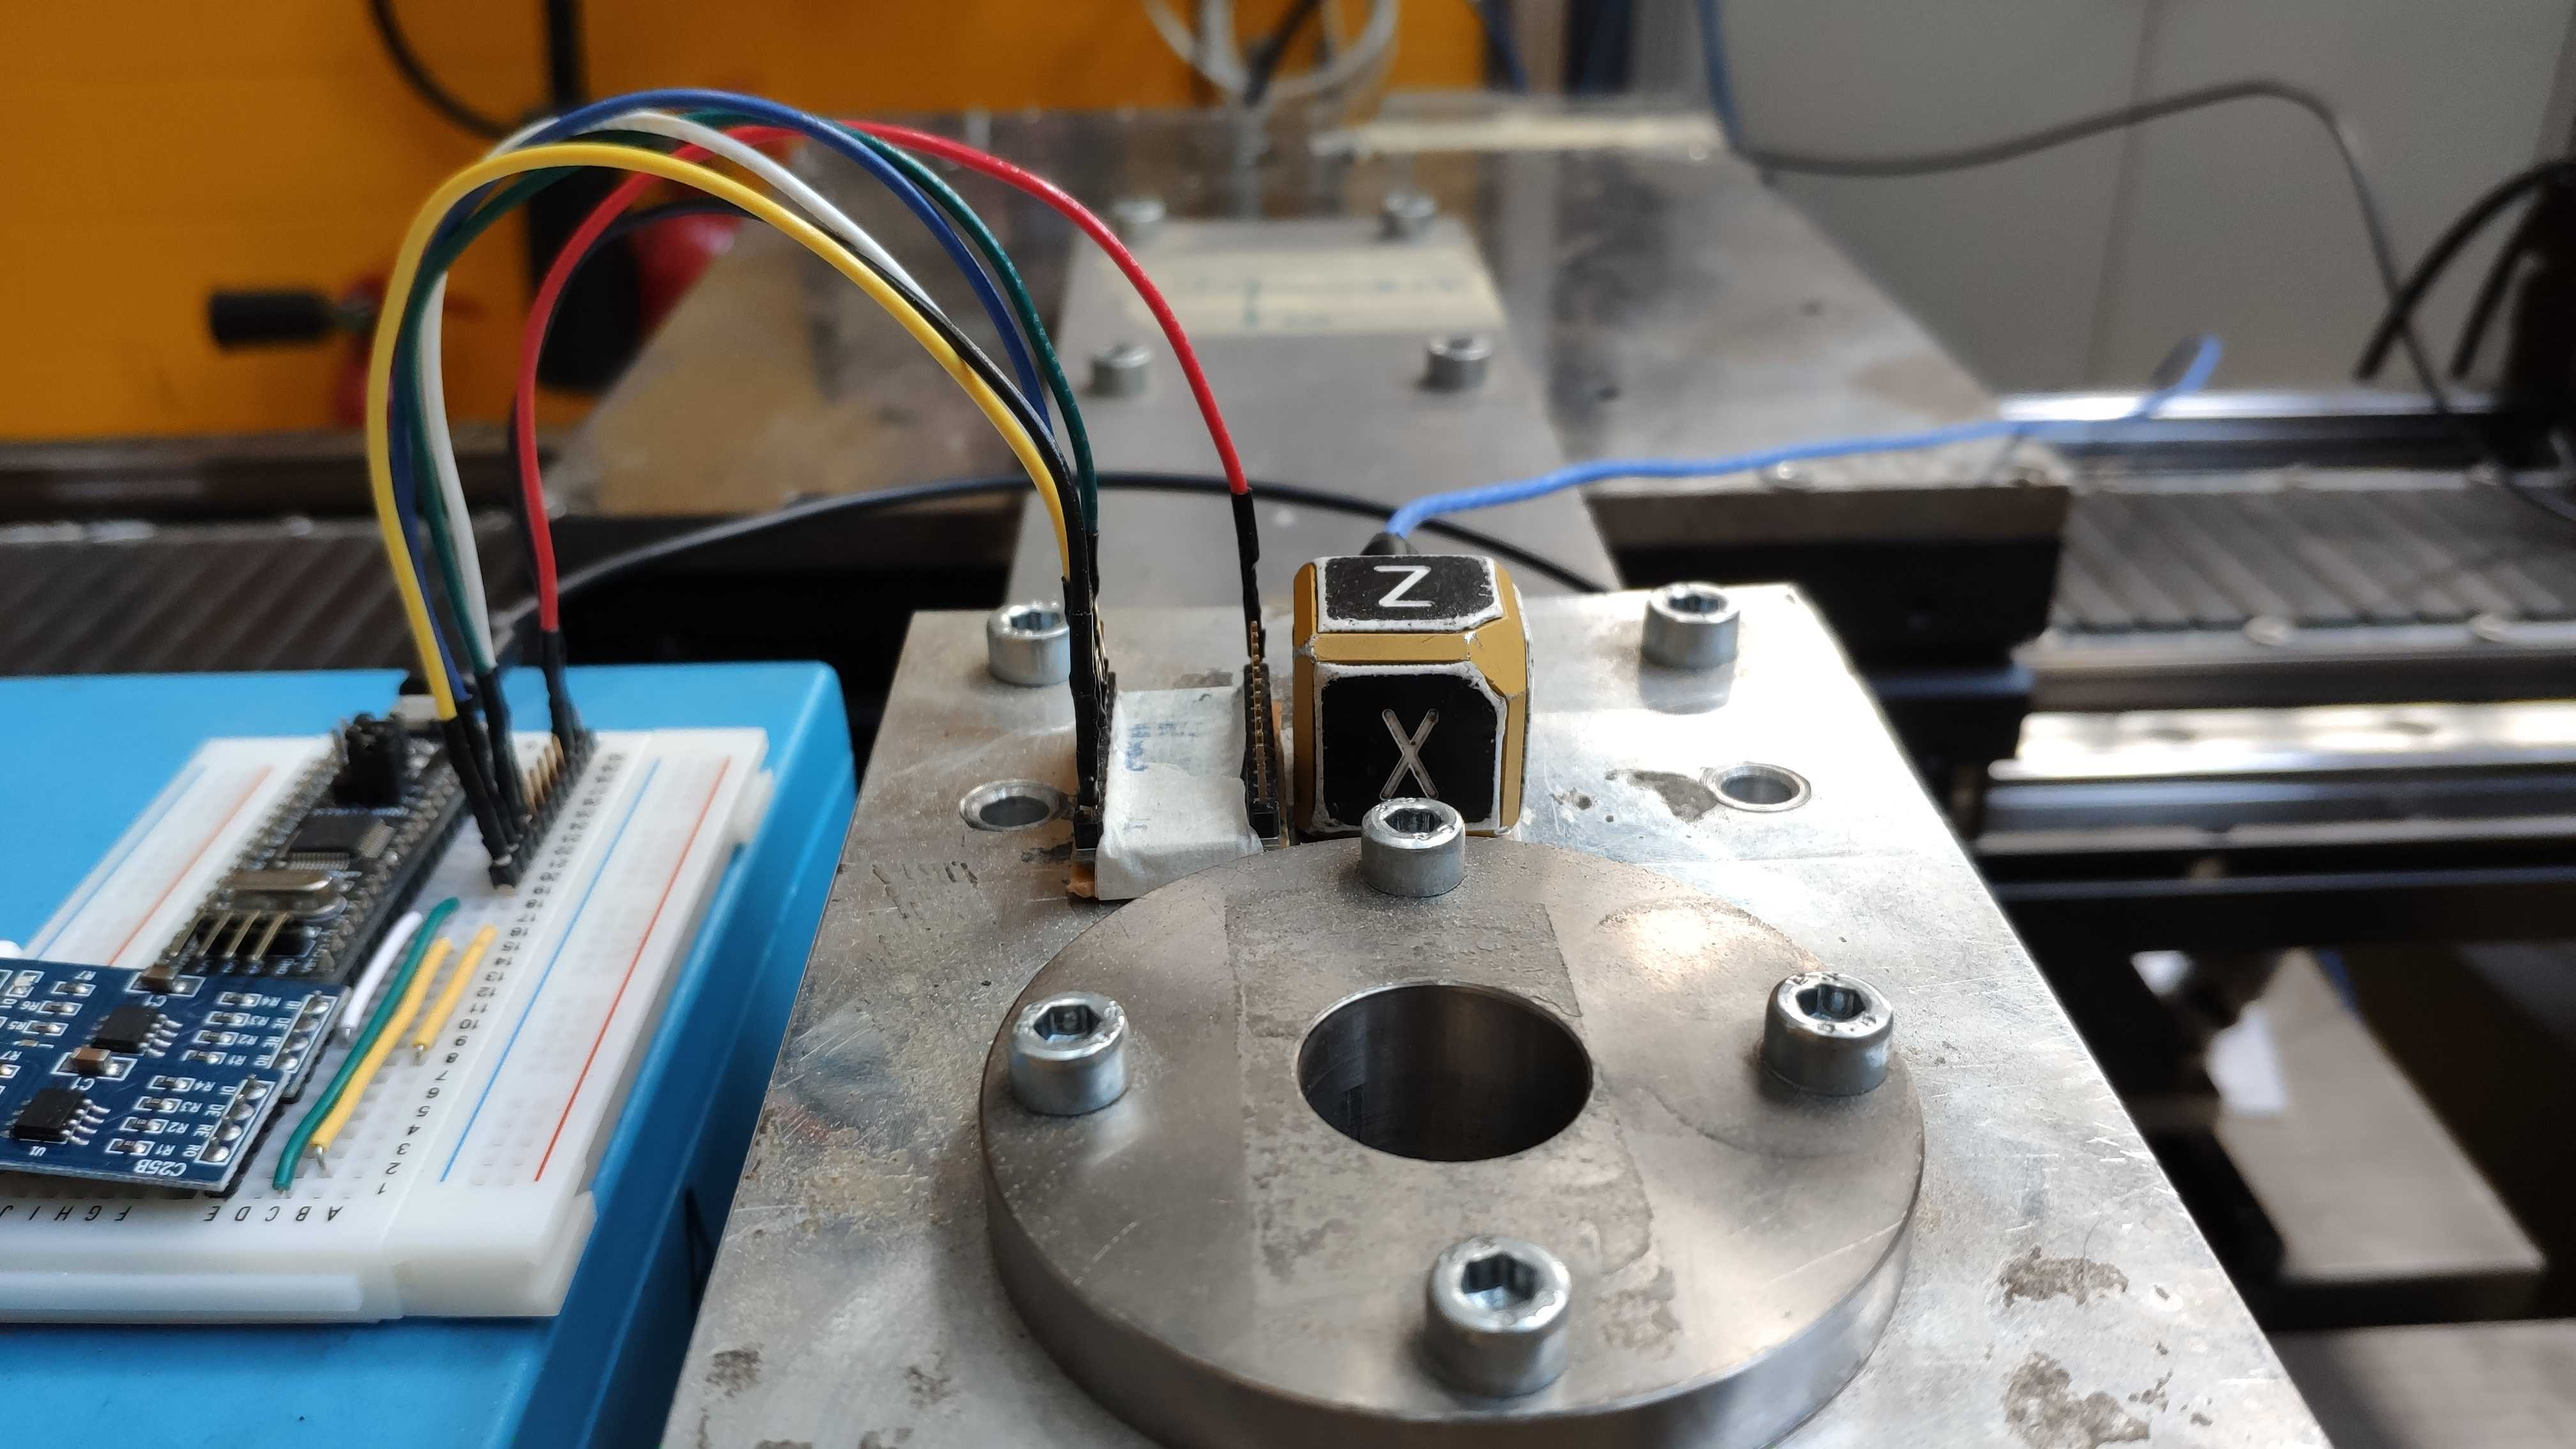
\includegraphics[width=0.3\linewidth]{figures/test_setups/Andromeda/Andromeda_Sensors.jpg}}
  \caption[Andromeda Test Setup]{Andromeda test setup%
    \label{fig:andromeda_pics}}
\end{figure}

\begin{figure}[!htb]
  \centering
  \subcaptionbox{Top view\label{sfig:Andromeda_Positions_Top}}{%
    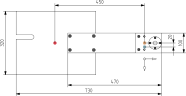
\includegraphics[scale=0.35]{figures/test_setups/Andromeda/Andromeda_Positions_Top}}
    \hspace{4em}
  \subcaptionbox{Trimetric view\label{sfig:Andromeda_Positions_Trimetric_coord}}{%
    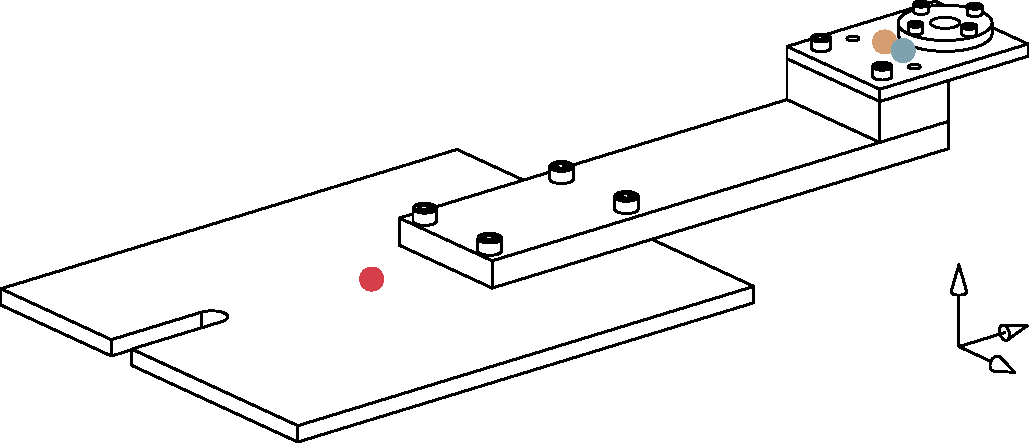
\includegraphics[scale=0.35]{figures/test_setups/Andromeda/Andromeda_Positions_Trimetric_coord}}
  \caption[Andromeda Example Positions]{Andromeda wagon, example impact position%
    \label{fig:andromeda_positions}}
\end{figure}

\section{Other Test Setups}

To test the bandwidth of the prototype \ac{LC} the hammer tip is hit against a rigid surface. The hardness of the hammer tip determines the bandwidth of the signal. And with hard tips the highest bandwidths can be explored. Apart from the signal measurement tests themselves other tests had to be conducted to guarantee the \ac{DAC} operation and to test the Software. As an example, clock tunable \ac{LPF} are tested in an arduino circuit, that generates a differential sinusoidal signal at different frequencies.


\chapter{Results and Discussion}
\label{chap:results}

results of the setups in \autoref{chp:test_setups} are discussed.

%***********************************
\section{Hammer-Hammer Test}

The results of the hammer-hammer test are impulse signal recordings of both, the reference system and the prototype \ac{LC}. Because the prototype signal is not calibrated, in order to able to compare the signals one needs to normalize the signal range of the reference signal. Furthermore, the signals need to be synced in time, by applying a time shift to one. The outputs gained after these transformations are shown in \figref{fig:HH_comparison}.

It can be seen that if one is using the soft PVC tip of the reference system both signals correlate well. If we then focus on the detailed view of such a test, as seen in \figref{fig:HH_noise}, the difference in resolution becomes apparent.

\begin{figure}[!htb]
  \centering
  \includestandalone[width=0.9\linewidth]{figures/test_setups/HH_comparison/HH_comparison}
  \caption[HH-Test comparison]{The HH-Test recordings of the reference hammer (orange) and the evaluated impact hammer system (turquoise). Note that the evaluated signal values are normalized so that the maxima are equal to the reference system.%
    \label{fig:HH_comparison}}
\end{figure}
\begin{figure}[!htb]
  \centering
  \includestandalone[width=\linewidth]{figures/test_setups/HH_noise/HH_noise}
  \caption[HH006 Plot]{Detailed plot of HH-Test 006%
    \label{fig:HH_noise}}
\end{figure}

\section{Andromeda Measurement}
Before comparing the accelerometer signals of the reference with the ones of the prototype system, one needs to subtract the constant gravitational part from the prototype signals. Additionally, the signals need to be synchronized in the time axis, as can be seen in \figref{fig:HAp024_TDat_z}.

When we then consider the frequency domain of \figref{fig:HAp024_FFTa_z} one can see that both signals cover the excited frequency bandwidth of around \SI{250}{\hertz} in a similar manner. The initial deviation at \SI{1}{\hertz} can be explained due to the signal conditioning in the reference system, where lower frequencies are cut-off.

\begin{figure}[!htb]
  \centering
  \includestandalone[width=0.8\linewidth]{figures/results/HAp024_TDat_z}
  \caption[Andromeda Measurement HAp024, Time Domain in Z-Axis]{Measurement HAp024 in the time domain, excitation at point A, as shown in \figref{fig:andromeda_positions}%
    \label{fig:HAp024_TDat_z}}
\end{figure}
\begin{figure}[!htb]
  \centering
  \includestandalone[width=0.8\linewidth]{figures/results/HAp024_FFTa_z}
  \caption[Andromeda Measurement HAp024, FFT in Z-Axis]{Measurement FFT HAp024, excitation at point A, as shown in \figref{fig:andromeda_positions}%
    \label{fig:HAp024_FFTa_z}}
\end{figure}

\section{Filter Test Setups}
The implementation of \figref{sfig:dac_comp_precond} is an iteration on the setup without a filter. But for the verification of the filter function a test setup was needed. But because of incompatibilites between the variable clock generator and the clock tunable filters, no meaningful output signals could be measured.

\chapter{Conclusion and Future Work}

%***********************************************************************
\section{Conclusion}
A force impact hammer has been constructed from only low-cost components. It has been demonstrated that a built in strain gauge load cell, which was designed for weighting applications, can follow the impulse trajectories with practically no overshoot. Said trajectory consistently follows the impulse of a reference piezoceramic apart from some expected increase in noise. The output signal of an experimental modal analysis measurement has been captured by a low-cost accelerometer which then showed a good correlation to a reference sensor. Furthermore, a microcontroller based data acquisition system has been developed with a specialized transmission protocol for microcontroller inter-communication. In this system, the use of a semi-duplex connections proved to decrease the reliability of the data acquisition.

\section{Progress and Points of Transfer}
Regarding the different layers of this project, it can be improved at multiples points. The filter has not been successfully implemented into the analog signal chain of the load cell yet. Neither were the clock tunable filters operational. As soon as the filter is integrated in the signal chain the upper bandwidth limit of the load cell can be tested with the use of harder hammer tips.
The data flow of the data acquisition system did not prove to be sufficiently reliable. Before multi-channeling accelerometers, one needs to consider to change the dataflow, for example by enabling daisy-chaining of the accelerometers.
One also can consider iterating the time synchronization.

%***********************************************************************
\section{Future Work}
The low-cost modal analysis system is not finished as it is. Multi-Channeling the accelerometer, industrializing, and eventually miniaturizing the product are the key next steps in the development. Of course testing, evaluating and comparing signals to a reference system and models will play an important role in guaranteeing the systems accuracy. Additionally, one can improve on what already exists, as described in the previous section. In the same way, we can also exchange components, adding different features. For example a better real time capability by switching from Arduino to a Raspberry Pi or even field programmable gate arrays. It is also possible to switch to wireless communication between nodes or test the limits of the current data bandwidth.

Our ultimate goal is to reduce costs of the modal analysis measurement procedure. Apart from the development of this system it will also become increasingly important to address the software interface and generally the handling of the device. Because it should become possible, that the specialists do not have to conduct the measurements themselves. For this, we need to make the device accessible to anyone with the use of thorough instructions and/or increased automation.



%Because, the system is not
%\begin{itemize}
%  \item Explore the same solution space further, i.e.\ handling the \ac{LPF} circuit and optimizing the software.
%  \item Change to a different solution space with either standard components using \ac{CPU}s or \ac{FPGA}s, targeting simpler implementation or higher bandwidths
%  \item Exploring the limits of the application and limits current solution without additional preconditioning
%\end{itemize}
%
%Independent of the chosen direction one can progress by
%\begin{itemize}
%  \item Testing the limits of multi channelling
%  \item Leaving the prototyping stage and simplify the production
%  \item Exploring wireless communication
%\end{itemize}


%%----------------------------------------------------------------
%% APPENDIX
\appendix\appendixtrue
\clearpage
\chapter{Appendix%
  \label{apx:appendix}}

\begin{figure}[!htb]
\sbox0{\subcaptionbox{Vertical stress, longitudinal particle displacement\label{sfig:piezo_beam}}{%
    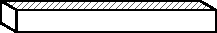
\includegraphics[scale=0.7]{figures/measurement/piezo/piezo_beam}
    }}% a
  \sbox1{\subcaptionbox{Vertical stress, lateral particle displacement\label{sfig:piezo_plate_top}}{%
    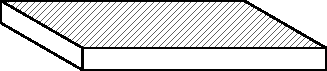
\includegraphics[scale=0.7]{figures/measurement/piezo/piezo_plate_top}
    }}% b
  \sbox2{\subcaptionbox{Vertical stress, lateral particle displacement\label{sfig:piezo_plate_side}}{%
    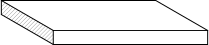
\includegraphics[scale=0.7]{figures/measurement/piezo/piezo_plate_side}
    }}% c
  \sbox3{\subcaptionbox{Lateral stress, lateral particle displacement\label{sfig:piezo_radial_long}}{%
    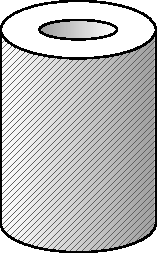
\includegraphics[scale=0.7]{figures/measurement/piezo/piezo_radial_long}
    }}% d
  \sbox4{\subcaptionbox{Radial particle displacement\label{sfig:piezo_radial_flat}}{%
    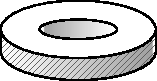
\includegraphics[scale=0.7]{figures/measurement/piezo/piezo_radial_flat}
    }}% e
  \sbox5{\subcaptionbox{Radial particle displacement\label{sfig:piezo_axial_hole_flat}}{%
    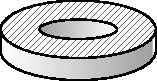
\includegraphics[scale=0.7]{figures/measurement/piezo/piezo_axial_hole_flat}
    }}% f
  \sbox6{\subcaptionbox{Vertical stress, radial particle displacement\label{sfig:piezo_sphere}}{%
    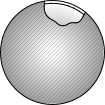
\includegraphics[scale=0.7]{figures/measurement/piezo/piezo_sphere}
    }}% g
  \sbox7{\subcaptionbox{Radial particle displacement\label{sfig:piezo_axial_flat}}{%
    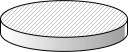
\includegraphics[scale=0.7]{figures/measurement/piezo/piezo_axial_flat}
    }}% h
  \sbox8{\subcaptionbox{Radial particle displacement\label{sfig:piezo_radial_rod}}{%
    
\includegraphics[scale=0.7]{figures/measurement/piezo/piezo_radial_rod}
    }}% i
  \centering
  {%
    \renewcommand{\arraystretch}{4}%
    \setlength{\tabcolsep}{2em}
    \begin{tabular}{ccc}
      \usebox0 & \usebox3 & \usebox6 \\
      \usebox1 & \usebox4 & \usebox7 \\
      \usebox2 & \usebox5 & \usebox8
    \end{tabular}
  }
  \caption[Piezoelectric designs]{Piezoelectric designs, where electrodes are placed on the shaded areas%
  \label{fig:piezo_designs}}
\end{figure}

\begin{figure}[!htb]
  \centering
  \includestandalone[scale=0.8]{figures/electronics/ic_flowchart/ic_flowchart}
  \caption[IC packages flowchart]{Flowchart of IC packages%
    \label{fig:ic_flowchart}}
\end{figure}
{\scriptsize%
\begin{longtable}{lccc}
\caption[Andromeda Measurements, Prototype Impact Hammer]{Andromeda measurement setup that is excited by the prototype impact hammer. The prototype accelerometer is set to a dynamic range of $\pm$\SI{16}{g} and a \acs{AAF} cut-off of \SI{800}{\hertz}.}\\
\toprule
Label & \makecell{Excitation\\Location} & \makecell{Prototype Sampling\\Rate / \si{\kilo\hertz}} & \makecell{Prototype Recording\\Duration / \si{\second}}\\
\midrule
\endfirsthead%
\caption[]{(Continued)}\\
\toprule
Label & \makecell{Excitation\\Location} & \makecell{Prototype Sampling\\Rate / \si{\kilo\hertz}} & \makecell{Prototype Recording\\Duration / \si{\second}}\\
\midrule
\endhead%
\midrule
\multicolumn{4}{c}{continued on next page}\\
\bottomrule
\endfoot%
%\bottomrule
\endlastfoot%
	HAe001 & A & 1.6 & 3\\
	HAe002 & A & 1.6 & 3\\
	HAe003 & A & 1.6 & 3\\
	HAe004 & A & 1.6 & 3\\
	HAe005 & A & 1.6 & 3\\
	HAe006 & B & 1.6 & 3\\
	HAe007 & B & 1.6 & 3\\
	HAe008 & B & 1.6 & 3\\
	HAe009 & B & 1.6 & 3\\
	HAe010 & B & 1.6 & 3\\
	HAe011 & C & 1.6 & 3\\
	HAe012 & C & 1.6 & 3\\
	HAe013 & C & 1.6 & 3\\
	HAe014 & C & 1.6 & 3\\
	HAe015 & C & 1.6 & 3\\
	HAe016 & D & 1.6 & 3\\
	HAe017 & D & 1.6 & 3\\
	HAe018 & D & 1.6 & 3\\
	HAe019 & D & 1.6 & 3\\
	HAe020 & D & 1.6 & 3\\
\bottomrule
\label{tab:hae_tests}
\end{longtable}
}

{\scriptsize%
\begin{longtable}{lccccc}
\caption[Andromeda Measurements, Reference Impact Hammer]{Andromeda measurement setup that is excited by the reference impact hammer}\\
\toprule
Label & \makecell{Excitation\\Location} & \makecell{Accelerometer Sampling\\Rate / \si{\kilo\hertz}} & \makecell{Prototype Recording\\Duration / \si{\second}} & \makecell{Accelrometer\\Dynamic Range / \si{g}} & \makecell{Accelerometer\\AAF cut-off / \si{\hertz}}\\
\midrule
\endfirsthead%
\caption[]{(Continued)}\\
\toprule
Label & \makecell{Excitation\\Location} & \makecell{Accelerometer Sampling\\Rate / \si{\kilo\hertz}} & \makecell{Prototype Recording\\Duration / \si{\second}} & \makecell{Accelrometer\\Dynamic Range / \si{g}} & \makecell{Accelerometer\\AAF cut-off / \si{\hertz}}\\
\midrule
\endhead%
\midrule
\multicolumn{6}{c}{continued on next page}\\
\bottomrule
\endfoot%
%\bottomrule
\endlastfoot%
  HAp001 & A & 1.6 & 3 & $\pm$16 & 800\\
	HAp002 & A & 1.6 & 3 & $\pm$16 & 800\\
	HAp003 & A & 1.6 & 3 & $\pm$16 & 800\\
	HAp004 & A & 1.6 & 3 & $\pm$16 & 800\\
	HAp005 & A & 1.6 & 3 & $\pm$16 & 800\\
	HAp006 & B & 1.6 & 3 & $\pm$16 & 800\\
	HAp007 & B & 1.6 & 3 & $\pm$16 & 800\\
	HAp008 & B & 1.6 & 3 & $\pm$16 & 800\\
	HAp009 & B & 1.6 & 3 & $\pm$16 & 800\\
	HAp010 & B & 1.6 & 3 & $\pm$16 & 800\\
	HAp011 & C & 1.6 & 3 & $\pm$16 & 800\\
	HAp012 & C & 1.6 & 3 & $\pm$16 & 800\\
	HAp013 & C & 1.6 & 3 & $\pm$16 & 800\\
	HAp014 & C & 1.6 & 3 & $\pm$16 & 800\\
	HAp015 & C & 1.6 & 3 & $\pm$16 & 800\\
	HAp016 & D & 1.6 & 3 & $\pm$16 & 800\\
	HAp017 & D & 1.6 & 3 & $\pm$16 & 800\\
	HAp018 & D & 1.6 & 3 & $\pm$16 & 800\\
	HAp019 & D & 1.6 & 3 & $\pm$16 & 800\\
	HAp020 & D & 1.6 & 3 & $\pm$16 & 800\\
	HAp001 & A & 0.8 & 3 & $\pm$16 & 400\\
	HAp002 & A & 0.8 & 3 & $\pm$16 & 400\\
	HAp003 & A & 0.8 & 3 & $\pm$16 & 400\\
	HAp004 & A & 0.8 & 3 & $\pm$16 & 400\\
	HAp005 & A & 0.8 & 3 & $\pm$16 & 400\\
	HAp006 & B & 0.8 & 3 & $\pm$16 & 400\\
	HAp007 & B & 0.8 & 3 & $\pm$16 & 400\\
	HAp008 & B & 0.8 & 3 & $\pm$16 & 400\\
	HAp009 & B & 0.8 & 3 & $\pm$16 & 400\\
	HAp010 & B & 0.8 & 3 & $\pm$16 & 400\\
	HAp011 & C & 0.8 & 3 & $\pm$16 & 400\\
	HAp012 & C & 0.8 & 3 & $\pm$16 & 400\\
	HAp013 & C & 0.8 & 3 & $\pm$16 & 400\\
	HAp014 & C & 0.8 & 3 & $\pm$16 & 400\\
	HAp015 & C & 0.8 & 3 & $\pm$16 & 400\\
	HAp016 & D & 0.8 & 3 & $\pm$16 & 400\\
	HAp017 & D & 0.8 & 3 & $\pm$16 & 400\\
	HAp018 & D & 0.8 & 3 & $\pm$16 & 400\\
	HAp019 & D & 0.8 & 3 & $\pm$16 & 400\\
	HAp020 & D & 0.8 & 3 & $\pm$16 & 400\\
	HAp021 & C & 1.6 & 3 & $\pm$4 & 800\\
	HAp022 & C & 1.6 & 3 & $\pm$4 & 800\\
	HAp023 & C & 1.6 & 3 & $\pm$4 & 800\\
	HAp024 & C & 1.6 & 3 & $\pm$4 & 800\\
	HAp025 & C & 1.6 & 3 & $\pm$4 & 800\\
	HAp026 & D & 1.6 & 3 & $\pm$2 & 800\\
	HAp027 & D & 1.6 & 3 & $\pm$2 & 800\\
	HAp028 & D & 1.6 & 3 & $\pm$4 & 800\\
	HAp029 & D & 1.6 & 3 & $\pm$4 & 800\\
	HAp030 & D & 1.6 & 3 & $\pm$4 & 800\\
\bottomrule
\label{tab:hap_tests}
\end{longtable}
}

{\scriptsize%
\begin{longtable}{lccc}
\caption[Hammer-Hammer Test Measurements]{Hammer-hammer test measurements}\\
\toprule
Label & \makecell{Prototype\\tip} & \makecell{Prototype Sampling\\Rate / \si{\kilo\hertz}} & \makecell{Prototype Recording\\Duration / \si{\second}}\\
\midrule
\endfirsthead%
\caption[]{(Continued)}\\
\toprule
Label & \makecell{Prototype\\tip} & \makecell{Prototype Sampling\\Rate / \si{\kilo\hertz}} & \makecell{Prototype Recording\\Duration / \si{\second}}\\
\midrule
\endhead%
\midrule
\multicolumn{4}{c}{continued on next page}\\
\bottomrule
\endfoot%
%\bottomrule
\endlastfoot%
\hline
	HH001 & 34CrMo4 & 3 & 4\\
	HH002 & 34CrMo4 & 3 & 4\\
	HH003 & 34CrMo4 & 3 & 4\\
	HH004 & 34CrMo4 & 3 & 4\\
	HH005 & 34CrMo4 & 3 & 4\\
	HH006 & 34CrMo4 & 3 & 4\\
	HH007 & 34CrMo4 & 3 & 4\\
	HH008 & 34CrMo4 & 3 & 4\\
	HH009 & 34CrMo4 & 3 & 4\\
	HH010 & 34CrMo4 & 3 & 4\\
	HH011 & 34CrMo4 & 3 & 3\\
	HH012 & 34CrMo4 & 2 & 3\\
	HH013 & 34CrMo4 & 2 & 3\\
	HH014 & 34CrMo4 & 2 & 3\\
	HH015 & 34CrMo4 & 2 & 3\\
	HH016 & Elastomer & 2 & 3\\
	HH017 & Elastomer & 2 & 3\\
	HH018 & Elastomer & 2 & 3\\
	HH019 & Elastomer & 2 & 3\\
	HH020 & Elastomer & 2 & 3\\
\bottomrule
\label{tab:hh_tests}
\end{longtable}
}

{\scriptsize%
\begin{longtable}{lccc}
\caption[Hammer-Surface Measurements]{Hammer-surface measurements}\\
\toprule
Label & \makecell{Prototype\\tip} & \makecell{Prototype Sampling\\Rate / \si{\kilo\hertz}} & \makecell{Prototype Recording\\Duration / \si{\second}}\\
\midrule
\endfirsthead%
\caption[]{(Continued)}\\
\toprule
Label & \makecell{Prototype\\tip} & \makecell{Prototype Sampling\\Rate / \si{\kilo\hertz}} & \makecell{Prototype Recording\\Duration / \si{\second}}\\
\midrule
\endhead%
\midrule
\multicolumn{4}{c}{continued on next page}\\
\bottomrule
\endfoot%
%\bottomrule
\endlastfoot%
	HS001 & 34CrMo4 & 2 & 1\\
	HS002 & 34CrMo4 & 2 & 1\\
	HS003 & 34CrMo4 & 2 & 1\\
	HS004 & 34CrMo4 & 2 & 1\\
	HS005 & 34CrMo4 & 2 & 1\\
	HS006 & 34CrMo4 & 2.5 & 1\\
	HS007 & 34CrMo4 & 2.5 & 1\\
	HS008 & 34CrMo4 & 2.5 & 1\\
	HS009 & 34CrMo4 & 2.5 & 1\\
	HS010 & 34CrMo4 & 2.5 & 1\\
	HS011 & 34CrMo4 & 1.67 & 1\\
	HS012 & 34CrMo4 & 1.67 & 1\\
	HS013 & 34CrMo4 & 1.67 & 1\\
	HS014 & 34CrMo4 & 1.67 & 1\\
	HS015 & 34CrMo4 & 1.67 & 1\\
	HS016 & Elastomer & 1.67 & 1\\
	HS017 & Elastomer & 1.67 & 1\\
	HS018 & Elastomer & 1.67 & 1\\
	HS019 & Elastomer & 1.67 & 1\\
	HS020 & Elastomer & 1.67 & 1\\
	HS021 & Elastomer & 2 & 1\\
	HS022 & Elastomer & 2 & 1\\
	HS023 & Elastomer & 2 & 1\\
	HS024 & Elastomer & 2 & 1\\
	HS025 & Elastomer & 2 & 1\\
	HS026 & Elastomer & 2.5 & 1\\
	HS027 & Elastomer & 2.5 & 1\\
	HS028 & Elastomer & 2.5 & 1\\
	HS029 & Elastomer & 2.5 & 1\\
	HS030 & Elastomer & 2.5 & 1\\
\bottomrule
\label{tab:hs_tests}
\end{longtable}
}


\begin{figure}[!htb]
  \centering
  \includestandalone[width=0.8\linewidth]{figures/results/HAp024_TDat_x}
  \caption[Andromeda Measurement HAp024, Time Domain in X-Axis]{Measurement HAp024 in the time domain, excitation at point A, as shown in \figref{fig:andromeda_positions}%
    \label{fig:HAp024_TDat_x}}
\end{figure}
\begin{figure}[!htb]
    \centering
    \includestandalone[width=0.8\linewidth]{figures/results/HAp024_FFTa_x}
    \caption[Andromeda Measurement HAp024, FFT in X-Axis]{Measurement FFT HAp024, excitation at point A, as shown in \figref{fig:andromeda_positions}%
      \label{fig:HAp024_FFTa_x}}
\end{figure}

\begin{figure}[!htb]
    \centering
    \includestandalone[width=0.8\linewidth]{figures/results/HAp024_TDat_y}
    \caption[Andromeda Measurement HAp024, Time Domain in Y-Axis]{Measurement HAp024 in the time domain, excitation at point A, as shown in \figref{fig:andromeda_positions}%
      \label{fig:HAp024_TDat_y}}
\end{figure}
\begin{figure}[!htb]
    \centering
    \includestandalone[width=0.8\linewidth]{figures/results/HAp024_FFTa_y}
    \caption[Andromeda Measurement HAp024, FFT in Y-Axis]{Measurement FFT HAp024, excitation at point A, as shown in \figref{fig:andromeda_positions}%
      \label{fig:HAp024_FFTa_y}}
\end{figure}


%%----------------------------------------------------------------
%% REFERENCES
\cleardoublepage
\phantomsection
% \renewcommand*{\chapterpagestyle}{empty}
\addcontentsline{toc}{chapter}{List of figures}
\listoffigures

\cleardoublepage
\phantomsection
\addcontentsline{toc}{chapter}{List of tables}
\listoftables

\cleardoublepage
\phantomsection
\clearpage
%\renewcommand*{\chapterpagestyle}{empty}
\addcontentsline{toc}{chapter}{Bibliography}
\printbibliography

\end{document}